\section{Iteracyjne metody rozwiązywania równań eliptycznych}

Będziemy korzystać z równania:

$$u_{i,j} = \frac{1}{4}(u_{i+1,j} + u_{i-1,j} + u_{i,j+1} + u_{i,j-1}) - \frac{1}{4}h^2f_{i,j}$$

\vspace{0.5cm}

Rozpatrzmy równanie:

\[
\begin{cases}
\vspace{0.1cm} 
\hspace{0,1cm}\dfrac{\partial^2 u}{\partial x^2} + \dfrac{\partial^2 u}{\partial y^2} = f\\
\vspace{0.1cm}
\hspace{0,1cm}u_{|\partial \Omega} = \widetilde{u} \\
\end{cases}
\]

, gdzie:

$(x,y) \in \Omega$

$\Omega = [a,b] \times [c,d]$

$\Omega \subset \Re^2$

\subsection{Cel ćwiczenia}

Naszym zadaniem było stworzenie algorytmu rozwiązującego następujące równania:

a) \hspace{6cm} b)

$\dfrac{\partial^2 u}{\partial x^2} + \dfrac{\partial^2 u}{\partial y^2} = 0$ \hspace{4.15cm} $\dfrac{\partial^2 u}{\partial x^2} + \dfrac{\partial^2 u}{\partial y^2} = -cos(x+y)-cos(x-y)$

, gdzie: \hspace{5.2cm} , gdzie:

warunki brzegowe: \hspace{3.5cm} warunki brzegowe:

$u(x,0) = 2lnx$ \hspace{4.15cm} $u(x,0) = cos(x)$

$u(1,y) = ln(y^2 + 1)$ \hspace{3.3cm} $u(0,y) = cos(y)$

$u(x,1) = ln(x^2 + 1)$ \hspace{3.28cm} $u(x,\frac{\pi}{2}) = 0$

$u(2,y) = ln(y^2 + 4)$ \hspace{3.3cm} $u(\pi,y) = -cos(y)$

rozwiązanie analityczne: \hspace{2.6cm} rozwiązanie analityczne:

$u(x,y) = ln(x^2 + y^2)$ \hspace{3.1cm} $u(x,y) = cos(x)\cdot cos(y)$

\vspace{0.5cm}

Trzema metodami: Jacobiego, Gaussa $-$ Seidela oraz nadrelaksacji Younge'a. Dodatkowo przedstawimy dwupoziomową metodę Peacemanna $-$ Rachforda.

\subsection{Metoda Jacobiego}

W metodzie tej wybieramy pierwsze arbitralne, dowolne przybliżenie rozwiązania numerycznego.

Im bliżej rozwiązania analitycznego dobrane jest przybliżenie tym mniej iteracji będziemy potrzebować w procesie iteracyjnym.

Jedna pełna iteracja polega na poprawieniu jeden raz wartości przybliżonych we wszystkich węzłach wewnętrznych siatki, aby następnie przejść do kolejnej iteracji wychodząc z tego samego węzła co poprzednio.

Dobór punktów nie ma znaczenia, ważne jest jedynie aby w kolejnych iteracjach zachować obrany porządek.

Zaletą metody Jacobiego jest nie generowanie wielkich macierzy; wadą dość wolna zbieżność.
\newpage
Dowolne pierwsze przybliżenie:

$$u_{i,j}^{(n)} = \frac{1}{4}(u_{i+1,j}^{(n)} + u_{i-1,j}^{(n)} + u_{i,j+1}^{(n)} + u_{i,j-1}^{(n)}) - \frac{1}{4}h^2f_{i,j}$$

\subsubsection{Algorytm}

a)

\documentclass[]{article}
\usepackage{lmodern}
\usepackage{amssymb,amsmath}
\usepackage{ifxetex,ifluatex}
\usepackage{fixltx2e} % provides \textsubscript
\ifnum 0\ifxetex 1\fi\ifluatex 1\fi=0 % if pdftex
  \usepackage[T1]{fontenc}
  \usepackage[utf8]{inputenc}
\else % if luatex or xelatex
  \ifxetex
    \usepackage{mathspec}
  \else
    \usepackage{fontspec}
  \fi
  \defaultfontfeatures{Ligatures=TeX,Scale=MatchLowercase}
\fi
% use upquote if available, for straight quotes in verbatim environments
\IfFileExists{upquote.sty}{\usepackage{upquote}}{}
% use microtype if available
\IfFileExists{microtype.sty}{%
\usepackage{microtype}
\UseMicrotypeSet[protrusion]{basicmath} % disable protrusion for tt fonts
}{}
\usepackage[margin=1in]{geometry}
\usepackage{hyperref}
\hypersetup{unicode=true,
            pdftitle={Lab5},
            pdfauthor={Me},
            pdfborder={0 0 0},
            breaklinks=true}
\urlstyle{same}  % don't use monospace font for urls
\usepackage{color}
\usepackage{fancyvrb}
\newcommand{\VerbBar}{|}
\newcommand{\VERB}{\Verb[commandchars=\\\{\}]}
\DefineVerbatimEnvironment{Highlighting}{Verbatim}{commandchars=\\\{\}}
% Add ',fontsize=\small' for more characters per line
\usepackage{framed}
\definecolor{shadecolor}{RGB}{248,248,248}
\newenvironment{Shaded}{\begin{snugshade}}{\end{snugshade}}
\newcommand{\KeywordTok}[1]{\textcolor[rgb]{0.13,0.29,0.53}{\textbf{{#1}}}}
\newcommand{\DataTypeTok}[1]{\textcolor[rgb]{0.13,0.29,0.53}{{#1}}}
\newcommand{\DecValTok}[1]{\textcolor[rgb]{0.00,0.00,0.81}{{#1}}}
\newcommand{\BaseNTok}[1]{\textcolor[rgb]{0.00,0.00,0.81}{{#1}}}
\newcommand{\FloatTok}[1]{\textcolor[rgb]{0.00,0.00,0.81}{{#1}}}
\newcommand{\ConstantTok}[1]{\textcolor[rgb]{0.00,0.00,0.00}{{#1}}}
\newcommand{\CharTok}[1]{\textcolor[rgb]{0.31,0.60,0.02}{{#1}}}
\newcommand{\SpecialCharTok}[1]{\textcolor[rgb]{0.00,0.00,0.00}{{#1}}}
\newcommand{\StringTok}[1]{\textcolor[rgb]{0.31,0.60,0.02}{{#1}}}
\newcommand{\VerbatimStringTok}[1]{\textcolor[rgb]{0.31,0.60,0.02}{{#1}}}
\newcommand{\SpecialStringTok}[1]{\textcolor[rgb]{0.31,0.60,0.02}{{#1}}}
\newcommand{\ImportTok}[1]{{#1}}
\newcommand{\CommentTok}[1]{\textcolor[rgb]{0.56,0.35,0.01}{\textit{{#1}}}}
\newcommand{\DocumentationTok}[1]{\textcolor[rgb]{0.56,0.35,0.01}{\textbf{\textit{{#1}}}}}
\newcommand{\AnnotationTok}[1]{\textcolor[rgb]{0.56,0.35,0.01}{\textbf{\textit{{#1}}}}}
\newcommand{\CommentVarTok}[1]{\textcolor[rgb]{0.56,0.35,0.01}{\textbf{\textit{{#1}}}}}
\newcommand{\OtherTok}[1]{\textcolor[rgb]{0.56,0.35,0.01}{{#1}}}
\newcommand{\FunctionTok}[1]{\textcolor[rgb]{0.00,0.00,0.00}{{#1}}}
\newcommand{\VariableTok}[1]{\textcolor[rgb]{0.00,0.00,0.00}{{#1}}}
\newcommand{\ControlFlowTok}[1]{\textcolor[rgb]{0.13,0.29,0.53}{\textbf{{#1}}}}
\newcommand{\OperatorTok}[1]{\textcolor[rgb]{0.81,0.36,0.00}{\textbf{{#1}}}}
\newcommand{\BuiltInTok}[1]{{#1}}
\newcommand{\ExtensionTok}[1]{{#1}}
\newcommand{\PreprocessorTok}[1]{\textcolor[rgb]{0.56,0.35,0.01}{\textit{{#1}}}}
\newcommand{\AttributeTok}[1]{\textcolor[rgb]{0.77,0.63,0.00}{{#1}}}
\newcommand{\RegionMarkerTok}[1]{{#1}}
\newcommand{\InformationTok}[1]{\textcolor[rgb]{0.56,0.35,0.01}{\textbf{\textit{{#1}}}}}
\newcommand{\WarningTok}[1]{\textcolor[rgb]{0.56,0.35,0.01}{\textbf{\textit{{#1}}}}}
\newcommand{\AlertTok}[1]{\textcolor[rgb]{0.94,0.16,0.16}{{#1}}}
\newcommand{\ErrorTok}[1]{\textcolor[rgb]{0.64,0.00,0.00}{\textbf{{#1}}}}
\newcommand{\NormalTok}[1]{{#1}}
\usepackage{graphicx,grffile}
\makeatletter
\def\maxwidth{\ifdim\Gin@nat@width>\linewidth\linewidth\else\Gin@nat@width\fi}
\def\maxheight{\ifdim\Gin@nat@height>\textheight\textheight\else\Gin@nat@height\fi}
\makeatother
% Scale images if necessary, so that they will not overflow the page
% margins by default, and it is still possible to overwrite the defaults
% using explicit options in \includegraphics[width, height, ...]{}
\setkeys{Gin}{width=\maxwidth,height=\maxheight,keepaspectratio}
\IfFileExists{parskip.sty}{%
\usepackage{parskip}
}{% else
\setlength{\parindent}{0pt}
\setlength{\parskip}{6pt plus 2pt minus 1pt}
}
\setlength{\emergencystretch}{3em}  % prevent overfull lines
\providecommand{\tightlist}{%
  \setlength{\itemsep}{0pt}\setlength{\parskip}{0pt}}
\setcounter{secnumdepth}{0}
% Redefines (sub)paragraphs to behave more like sections
\ifx\paragraph\undefined\else
\let\oldparagraph\paragraph
\renewcommand{\paragraph}[1]{\oldparagraph{#1}\mbox{}}
\fi
\ifx\subparagraph\undefined\else
\let\oldsubparagraph\subparagraph
\renewcommand{\subparagraph}[1]{\oldsubparagraph{#1}\mbox{}}
\fi

%%% Use protect on footnotes to avoid problems with footnotes in titles
\let\rmarkdownfootnote\footnote%
\def\footnote{\protect\rmarkdownfootnote}

%%% Change title format to be more compact
\usepackage{titling}

% Create subtitle command for use in maketitle
\newcommand{\subtitle}[1]{
  \posttitle{
    \begin{center}\large#1\end{center}
    }
}

\setlength{\droptitle}{-2em}

  \title{Lab5}
    \pretitle{\vspace{\droptitle}\centering\huge}
  \posttitle{\par}
    \author{Me}
    \preauthor{\centering\large\emph}
  \postauthor{\par}
      \predate{\centering\large\emph}
  \postdate{\par}
    \date{16 grudnia 2018}


\begin{document}
\maketitle

\begin{Shaded}
\begin{Highlighting}[]
\CommentTok{%metoda Jacobiego}
\FunctionTok{clc}
\FunctionTok{clear} \FunctionTok{all}
\FunctionTok{tic}

\CommentTok{%funkcja}
\NormalTok{F = @(x,y) }\FloatTok{0}\NormalTok{;}

\CommentTok{%rozwi?zanie analityczne}
\NormalTok{G = @(x,y) }\FunctionTok{log}\NormalTok{(x.^}\FloatTok{2}\NormalTok{+y.^}\FloatTok{2}\NormalTok{);}

\CommentTok{%przedzia? omega}
\NormalTok{xa=}\FloatTok{1}\NormalTok{;}
\NormalTok{xb=}\FloatTok{2}\NormalTok{;}
\NormalTok{yc=}\FloatTok{0}\NormalTok{;}
\NormalTok{yd=}\FloatTok{1}\NormalTok{;}

\CommentTok{%warunki brzegowe}
\NormalTok{u1 = @(x) }\FloatTok{2}\NormalTok{*}\FunctionTok{log}\NormalTok{(x);}
\NormalTok{u2 = @(y) }\FunctionTok{log}\NormalTok{(y.^}\FloatTok{2}\NormalTok{+}\FloatTok{4}\NormalTok{);}
\NormalTok{u3 = @(x) }\FunctionTok{log}\NormalTok{(x.^}\FloatTok{2}\NormalTok{+}\FloatTok{1}\NormalTok{);}
\NormalTok{u4 = @(y) }\FunctionTok{log}\NormalTok{(y.^}\FloatTok{2}\NormalTok{+}\FloatTok{1}\NormalTok{);}

\CommentTok{%siatka}
\NormalTok{n=}\FloatTok{5}\NormalTok{;}

\NormalTok{h=(xb-xa)/(n+}\FloatTok{1}\NormalTok{);}
\NormalTok{k=(yd-yc)/(n+}\FloatTok{1}\NormalTok{);}
\NormalTok{x=[xa:h:xb];}
\NormalTok{y=[yc:k:yd];}

\NormalTok{tol=}\FloatTok{1e-4}\NormalTok{; }
\FunctionTok{error} \NormalTok{= }\FloatTok{1}\NormalTok{; }
\NormalTok{licznik=}\FloatTok{0}\NormalTok{; }

\CommentTok{%tworzenie macierzy}
\NormalTok{for }\BaseNTok{i}\NormalTok{=}\FloatTok{1}\NormalTok{:n+}\FloatTok{2}
    \NormalTok{U(}\BaseNTok{i}\NormalTok{,}\FloatTok{1}\NormalTok{)=}\FloatTok{2}\NormalTok{*}\FunctionTok{log}\NormalTok{(xa+(}\BaseNTok{i}\NormalTok{-}\FloatTok{1}\NormalTok{)*h);}
    \NormalTok{U(}\FloatTok{1}\NormalTok{,}\BaseNTok{i}\NormalTok{)=}\FunctionTok{log}\NormalTok{(((yc+(}\BaseNTok{i}\NormalTok{-}\FloatTok{1}\NormalTok{)*k)^}\FloatTok{2}\NormalTok{)+}\FloatTok{1}\NormalTok{);}
\NormalTok{end}

\NormalTok{for }\BaseNTok{i}\NormalTok{=}\FloatTok{2}\NormalTok{:n+}\FloatTok{2}
    \NormalTok{U(}\BaseNTok{i}\NormalTok{,n+}\FloatTok{2}\NormalTok{)=}\FunctionTok{log}\NormalTok{(((xa+(}\BaseNTok{i}\NormalTok{-}\FloatTok{1}\NormalTok{)*h)^}\FloatTok{2}\NormalTok{)+}\FloatTok{1}\NormalTok{);}
    \NormalTok{U(n+}\FloatTok{2}\NormalTok{,}\BaseNTok{i}\NormalTok{)=}\FunctionTok{log}\NormalTok{(((yc+(}\BaseNTok{i}\NormalTok{-}\FloatTok{1}\NormalTok{)*k)^}\FloatTok{2}\NormalTok{)+}\FloatTok{4}\NormalTok{);}
\NormalTok{end}

\NormalTok{Uk=U;}

\NormalTok{while }\FunctionTok{error}\NormalTok{>tol}
    \NormalTok{licznik = licznik+}\FloatTok{1}\NormalTok{;}
    \NormalTok{for }\BaseNTok{i}\NormalTok{=}\FloatTok{2}\NormalTok{:n+}\FloatTok{1}
        \NormalTok{for }\BaseNTok{j}\NormalTok{=}\FloatTok{2}\NormalTok{:n+}\FloatTok{1}
            \NormalTok{Uk(}\BaseNTok{i}\NormalTok{,}\BaseNTok{j}\NormalTok{) =}\FloatTok{0.25}\NormalTok{*(U(}\BaseNTok{i}\NormalTok{+}\FloatTok{1}\NormalTok{,}\BaseNTok{j}\NormalTok{)+U(}\BaseNTok{i}\NormalTok{-}\FloatTok{1}\NormalTok{,}\BaseNTok{j}\NormalTok{)+U(}\BaseNTok{i}\NormalTok{,}\BaseNTok{j}\NormalTok{+}\FloatTok{1}\NormalTok{)+U(}\BaseNTok{i}\NormalTok{,}\BaseNTok{j}\NormalTok{-}\FloatTok{1}\NormalTok{))-}\FloatTok{0.25}\NormalTok{*h^}\FloatTok{2}\NormalTok{*F(x(}\BaseNTok{i}\NormalTok{),y(}\BaseNTok{j}\NormalTok{));}
        \NormalTok{end}
    \NormalTok{end}
    
    \FunctionTok{error} \NormalTok{= }\FunctionTok{max}\NormalTok{(}\FunctionTok{max}\NormalTok{(}\FunctionTok{abs}\NormalTok{(Uk-U)));}

    \NormalTok{U=Uk;}
\NormalTok{end}

\CommentTok{%wykresy}
\NormalTok{[X,Y] = }\FunctionTok{meshgrid}\NormalTok{(x,y);}
\FunctionTok{subplot}\NormalTok{(}\FloatTok{1}\NormalTok{,}\FloatTok{2}\NormalTok{,}\FloatTok{1}\NormalTok{)}
\FunctionTok{surf}\NormalTok{(X,Y,U')}
\FunctionTok{title}\NormalTok{(}\StringTok{'Metoda Numeryczna'}\NormalTok{)}
\FunctionTok{subplot}\NormalTok{(}\FloatTok{1}\NormalTok{,}\FloatTok{2}\NormalTok{,}\FloatTok{2}\NormalTok{)}
\FunctionTok{surf}\NormalTok{(X,Y,(G(X,Y)))}
\FunctionTok{title}\NormalTok{(}\StringTok{'Metoda Analityczna'}\NormalTok{)}

\NormalTok{blad = }\FunctionTok{max}\NormalTok{(}\FunctionTok{max}\NormalTok{(}\FunctionTok{abs}\NormalTok{(U'-G(X,Y))))}
\NormalTok{licznik}
\FunctionTok{toc}
\end{Highlighting}
\end{Shaded}

\begin{verbatim}
## blad =    8.1538e-04
## licznik =  54
## Elapsed time is 0.283208 seconds.
\end{verbatim}


\end{document}

\newpage
b)

\documentclass[]{article}
\usepackage{lmodern}
\usepackage{amssymb,amsmath}
\usepackage{ifxetex,ifluatex}
\usepackage{fixltx2e} % provides \textsubscript
\ifnum 0\ifxetex 1\fi\ifluatex 1\fi=0 % if pdftex
  \usepackage[T1]{fontenc}
  \usepackage[utf8]{inputenc}
\else % if luatex or xelatex
  \ifxetex
    \usepackage{mathspec}
  \else
    \usepackage{fontspec}
  \fi
  \defaultfontfeatures{Ligatures=TeX,Scale=MatchLowercase}
\fi
% use upquote if available, for straight quotes in verbatim environments
\IfFileExists{upquote.sty}{\usepackage{upquote}}{}
% use microtype if available
\IfFileExists{microtype.sty}{%
\usepackage{microtype}
\UseMicrotypeSet[protrusion]{basicmath} % disable protrusion for tt fonts
}{}
\usepackage[margin=1in]{geometry}
\usepackage{hyperref}
\hypersetup{unicode=true,
            pdftitle={Lab5},
            pdfauthor={Me},
            pdfborder={0 0 0},
            breaklinks=true}
\urlstyle{same}  % don't use monospace font for urls
\usepackage{color}
\usepackage{fancyvrb}
\newcommand{\VerbBar}{|}
\newcommand{\VERB}{\Verb[commandchars=\\\{\}]}
\DefineVerbatimEnvironment{Highlighting}{Verbatim}{commandchars=\\\{\}}
% Add ',fontsize=\small' for more characters per line
\usepackage{framed}
\definecolor{shadecolor}{RGB}{248,248,248}
\newenvironment{Shaded}{\begin{snugshade}}{\end{snugshade}}
\newcommand{\KeywordTok}[1]{\textcolor[rgb]{0.13,0.29,0.53}{\textbf{{#1}}}}
\newcommand{\DataTypeTok}[1]{\textcolor[rgb]{0.13,0.29,0.53}{{#1}}}
\newcommand{\DecValTok}[1]{\textcolor[rgb]{0.00,0.00,0.81}{{#1}}}
\newcommand{\BaseNTok}[1]{\textcolor[rgb]{0.00,0.00,0.81}{{#1}}}
\newcommand{\FloatTok}[1]{\textcolor[rgb]{0.00,0.00,0.81}{{#1}}}
\newcommand{\ConstantTok}[1]{\textcolor[rgb]{0.00,0.00,0.00}{{#1}}}
\newcommand{\CharTok}[1]{\textcolor[rgb]{0.31,0.60,0.02}{{#1}}}
\newcommand{\SpecialCharTok}[1]{\textcolor[rgb]{0.00,0.00,0.00}{{#1}}}
\newcommand{\StringTok}[1]{\textcolor[rgb]{0.31,0.60,0.02}{{#1}}}
\newcommand{\VerbatimStringTok}[1]{\textcolor[rgb]{0.31,0.60,0.02}{{#1}}}
\newcommand{\SpecialStringTok}[1]{\textcolor[rgb]{0.31,0.60,0.02}{{#1}}}
\newcommand{\ImportTok}[1]{{#1}}
\newcommand{\CommentTok}[1]{\textcolor[rgb]{0.56,0.35,0.01}{\textit{{#1}}}}
\newcommand{\DocumentationTok}[1]{\textcolor[rgb]{0.56,0.35,0.01}{\textbf{\textit{{#1}}}}}
\newcommand{\AnnotationTok}[1]{\textcolor[rgb]{0.56,0.35,0.01}{\textbf{\textit{{#1}}}}}
\newcommand{\CommentVarTok}[1]{\textcolor[rgb]{0.56,0.35,0.01}{\textbf{\textit{{#1}}}}}
\newcommand{\OtherTok}[1]{\textcolor[rgb]{0.56,0.35,0.01}{{#1}}}
\newcommand{\FunctionTok}[1]{\textcolor[rgb]{0.00,0.00,0.00}{{#1}}}
\newcommand{\VariableTok}[1]{\textcolor[rgb]{0.00,0.00,0.00}{{#1}}}
\newcommand{\ControlFlowTok}[1]{\textcolor[rgb]{0.13,0.29,0.53}{\textbf{{#1}}}}
\newcommand{\OperatorTok}[1]{\textcolor[rgb]{0.81,0.36,0.00}{\textbf{{#1}}}}
\newcommand{\BuiltInTok}[1]{{#1}}
\newcommand{\ExtensionTok}[1]{{#1}}
\newcommand{\PreprocessorTok}[1]{\textcolor[rgb]{0.56,0.35,0.01}{\textit{{#1}}}}
\newcommand{\AttributeTok}[1]{\textcolor[rgb]{0.77,0.63,0.00}{{#1}}}
\newcommand{\RegionMarkerTok}[1]{{#1}}
\newcommand{\InformationTok}[1]{\textcolor[rgb]{0.56,0.35,0.01}{\textbf{\textit{{#1}}}}}
\newcommand{\WarningTok}[1]{\textcolor[rgb]{0.56,0.35,0.01}{\textbf{\textit{{#1}}}}}
\newcommand{\AlertTok}[1]{\textcolor[rgb]{0.94,0.16,0.16}{{#1}}}
\newcommand{\ErrorTok}[1]{\textcolor[rgb]{0.64,0.00,0.00}{\textbf{{#1}}}}
\newcommand{\NormalTok}[1]{{#1}}
\usepackage{graphicx,grffile}
\makeatletter
\def\maxwidth{\ifdim\Gin@nat@width>\linewidth\linewidth\else\Gin@nat@width\fi}
\def\maxheight{\ifdim\Gin@nat@height>\textheight\textheight\else\Gin@nat@height\fi}
\makeatother
% Scale images if necessary, so that they will not overflow the page
% margins by default, and it is still possible to overwrite the defaults
% using explicit options in \includegraphics[width, height, ...]{}
\setkeys{Gin}{width=\maxwidth,height=\maxheight,keepaspectratio}
\IfFileExists{parskip.sty}{%
\usepackage{parskip}
}{% else
\setlength{\parindent}{0pt}
\setlength{\parskip}{6pt plus 2pt minus 1pt}
}
\setlength{\emergencystretch}{3em}  % prevent overfull lines
\providecommand{\tightlist}{%
  \setlength{\itemsep}{0pt}\setlength{\parskip}{0pt}}
\setcounter{secnumdepth}{0}
% Redefines (sub)paragraphs to behave more like sections
\ifx\paragraph\undefined\else
\let\oldparagraph\paragraph
\renewcommand{\paragraph}[1]{\oldparagraph{#1}\mbox{}}
\fi
\ifx\subparagraph\undefined\else
\let\oldsubparagraph\subparagraph
\renewcommand{\subparagraph}[1]{\oldsubparagraph{#1}\mbox{}}
\fi

%%% Use protect on footnotes to avoid problems with footnotes in titles
\let\rmarkdownfootnote\footnote%
\def\footnote{\protect\rmarkdownfootnote}

%%% Change title format to be more compact
\usepackage{titling}

% Create subtitle command for use in maketitle
\newcommand{\subtitle}[1]{
  \posttitle{
    \begin{center}\large#1\end{center}
    }
}

\setlength{\droptitle}{-2em}

  \title{Lab5}
    \pretitle{\vspace{\droptitle}\centering\huge}
  \posttitle{\par}
    \author{Me}
    \preauthor{\centering\large\emph}
  \postauthor{\par}
      \predate{\centering\large\emph}
  \postdate{\par}
    \date{16 grudnia 2018}


\begin{document}
\maketitle

\begin{Shaded}
\begin{Highlighting}[]
\CommentTok{%metoda Jacobiego}
\FunctionTok{clc}
\FunctionTok{clear} \FunctionTok{all}
\FunctionTok{tic}

\CommentTok{%funkcja}
\NormalTok{F = @(x,y) -}\FunctionTok{cos}\NormalTok{(x+y)-}\FunctionTok{cos}\NormalTok{(x-y);}

\CommentTok{%rozwi?zanie analityczne}
\NormalTok{G = @(x,y) }\FunctionTok{cos}\NormalTok{(x).*}\FunctionTok{cos}\NormalTok{(y);}

\CommentTok{%przedzia? omega}
\NormalTok{xa=}\FloatTok{0}\NormalTok{;}
\NormalTok{xb=}\BaseNTok{pi}\NormalTok{;}
\NormalTok{yc=}\FloatTok{0}\NormalTok{;}
\NormalTok{yd=}\BaseNTok{pi}\NormalTok{/}\FloatTok{2}\NormalTok{;}

\CommentTok{%warunki brzegowe}
\NormalTok{u1 = @(x) }\FunctionTok{cos}\NormalTok{(x);}
\NormalTok{u2 = @(y) -}\FunctionTok{cos}\NormalTok{(y);}
\NormalTok{u3 = @(x) }\FloatTok{0}\NormalTok{;}
\NormalTok{u4 = @(y) }\FunctionTok{cos}\NormalTok{(y);}

\CommentTok{%siatka}
\NormalTok{n=}\FloatTok{5}\NormalTok{;}

\NormalTok{h=(xb-xa)/(n+}\FloatTok{1}\NormalTok{);}
\NormalTok{k=(yd-yc)/(xb-xa)*(n+}\FloatTok{1}\NormalTok{)-}\FloatTok{1}\NormalTok{;}
\NormalTok{x=[xa:h:xb];}
\NormalTok{y=[yc:h:yd];}

\NormalTok{tol=}\FloatTok{1e-4}\NormalTok{;}
\FunctionTok{error} \NormalTok{= }\FloatTok{1}\NormalTok{; }
\NormalTok{licznik=}\FloatTok{0}\NormalTok{; }

\CommentTok{%tworzenie macierzy}
\NormalTok{U1(}\FloatTok{1}\NormalTok{:n+}\FloatTok{2}\NormalTok{) = u1(x);}
\NormalTok{U2(}\FloatTok{1}\NormalTok{:k+}\FloatTok{2}\NormalTok{) = u2(y(}\FloatTok{1}\NormalTok{:(k+}\FloatTok{2}\NormalTok{)));}
\NormalTok{U3(}\FloatTok{1}\NormalTok{:n+}\FloatTok{2}\NormalTok{) = u3(x);}
\NormalTok{U4(}\FloatTok{1}\NormalTok{:k+}\FloatTok{2}\NormalTok{) = u4(y(}\FloatTok{1}\NormalTok{:(k+}\FloatTok{2}\NormalTok{)));}

\NormalTok{U(}\FloatTok{1}\NormalTok{,:) = U1(}\FloatTok{1}\NormalTok{:n+}\FloatTok{2}\NormalTok{);}
\NormalTok{U(k+}\FloatTok{2}\NormalTok{,:) = U3(}\FloatTok{1}\NormalTok{:n+}\FloatTok{2}\NormalTok{);}
\NormalTok{U(:,}\FloatTok{1}\NormalTok{) = U4(}\FloatTok{1}\NormalTok{:k+}\FloatTok{2}\NormalTok{);}
\NormalTok{U(:,n+}\FloatTok{2}\NormalTok{) = U2(}\FloatTok{1}\NormalTok{:k+}\FloatTok{2}\NormalTok{);}

\NormalTok{Uk=U;}

\NormalTok{while }\FunctionTok{error}\NormalTok{>tol}
    \NormalTok{licznik = licznik+}\FloatTok{1}\NormalTok{;}
    \NormalTok{for }\BaseNTok{i}\NormalTok{=}\FloatTok{2}\NormalTok{:k+}\FloatTok{1}
        \NormalTok{for }\BaseNTok{j}\NormalTok{=}\FloatTok{2}\NormalTok{:n+}\FloatTok{1}
            \NormalTok{Uk(}\BaseNTok{i}\NormalTok{,}\BaseNTok{j}\NormalTok{) =}\FloatTok{0.25}\NormalTok{*(U(}\BaseNTok{i}\NormalTok{+}\FloatTok{1}\NormalTok{,}\BaseNTok{j}\NormalTok{)+U(}\BaseNTok{i}\NormalTok{-}\FloatTok{1}\NormalTok{,}\BaseNTok{j}\NormalTok{)+U(}\BaseNTok{i}\NormalTok{,}\BaseNTok{j}\NormalTok{+}\FloatTok{1}\NormalTok{)+U(}\BaseNTok{i}\NormalTok{,}\BaseNTok{j}\NormalTok{-}\FloatTok{1}\NormalTok{))-}\FloatTok{0.25}\NormalTok{*h^}\FloatTok{2}\NormalTok{*F(x(}\BaseNTok{j}\NormalTok{),y(}\BaseNTok{i}\NormalTok{));}
        \NormalTok{end}
    \NormalTok{end}
    
    \FunctionTok{error} \NormalTok{= }\FunctionTok{max}\NormalTok{(}\FunctionTok{max}\NormalTok{(}\FunctionTok{abs}\NormalTok{(Uk-U)));}

    \NormalTok{U=Uk;}
\NormalTok{end}

\CommentTok{%wykresy}
\NormalTok{[X,Y] = }\FunctionTok{meshgrid}\NormalTok{(x,y);}
\FunctionTok{subplot}\NormalTok{(}\FloatTok{1}\NormalTok{,}\FloatTok{2}\NormalTok{,}\FloatTok{1}\NormalTok{)}
\FunctionTok{surf}\NormalTok{(X,Y,U)}
\FunctionTok{title}\NormalTok{(}\StringTok{'Metoda Numeryczna'}\NormalTok{)}
\FunctionTok{subplot}\NormalTok{(}\FloatTok{1}\NormalTok{,}\FloatTok{2}\NormalTok{,}\FloatTok{2}\NormalTok{)}
\FunctionTok{surf}\NormalTok{(X,Y,(G(X,Y)))}
\FunctionTok{title}\NormalTok{(}\StringTok{'Metoda Analityczna'}\NormalTok{)}

\NormalTok{blad = }\FunctionTok{max}\NormalTok{(}\FunctionTok{max}\NormalTok{(}\FunctionTok{abs}\NormalTok{(U-G(X,Y))))}
\NormalTok{licznik}
\FunctionTok{toc}
\end{Highlighting}
\end{Shaded}

\begin{verbatim}
## blad =  0.0036873
## licznik =  13
## Elapsed time is 0.230382 seconds.
\end{verbatim}


\end{document}

\newpage
\subsubsection{Wykresy}

a)

Dla n = 5:

\begin{figure}[!ht]
	\begin{center}
		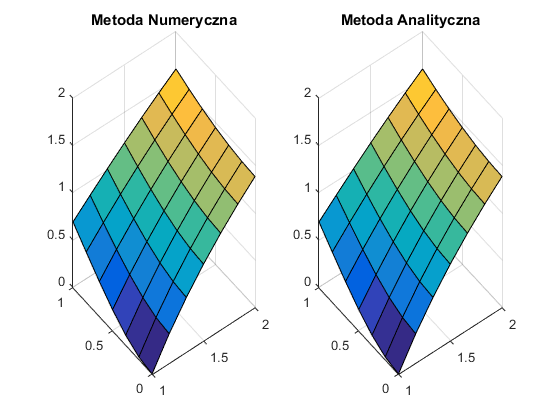
\includegraphics[width=0.78\textwidth]{Lab6/charts/jacobi/zad1/5.png}
	\end{center}
\end{figure}

Liczba wykonanych iteracji $ = 38 $

Czas wykonywania algorytmu $ = 0.177 s$


Dla n = 15:

\begin{figure}[!ht]
	\begin{center}
		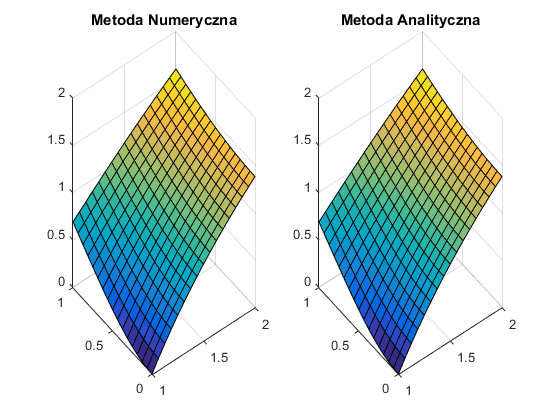
\includegraphics[width=0.78\textwidth]{Lab6/charts/jacobi/zad1/15.png}
	\end{center}
\end{figure}


Liczba wykonanych iteracji $ = 170 $

Czas wykonywania algorytmu $ = 0.202 s$
\newpage
Dla n = 30:

\begin{figure}[!ht]
	\begin{center}
		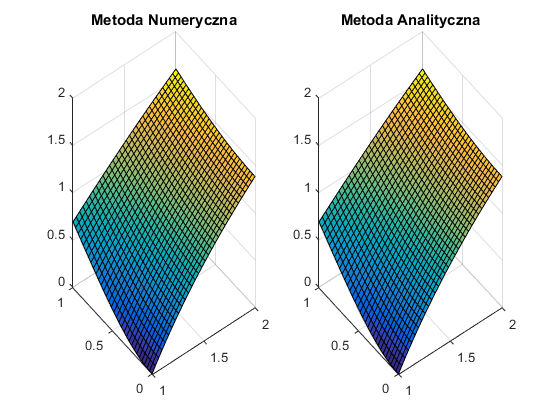
\includegraphics[width=0.8\textwidth]{Lab6/charts/jacobi/zad1/30.png}
	\end{center}
\end{figure}

Liczba wykonanych iteracji $ = 415 $

Czas wykonywania algorytmu $ = 0.289 s$



Dla n = 50:

\begin{figure}[!ht]
	\begin{center}
		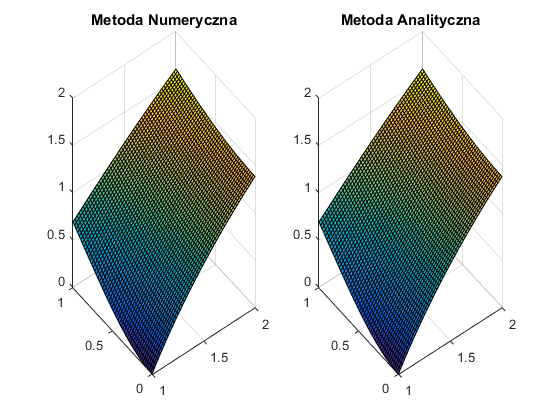
\includegraphics[width=0.8\textwidth]{Lab6/charts/jacobi/zad1/50.png}
	\end{center}
\end{figure}

Liczba wykonanych iteracji $ = 797 $

Czas wykonywania algorytmu $ = 0.777 s$
\newpage
b)

Dla n = 5:

\begin{figure}[!ht]
	\begin{center}
		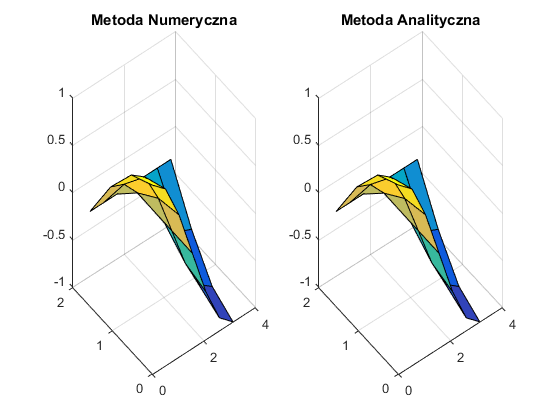
\includegraphics[width=0.8\textwidth]{Lab6/charts/jacobi/zad2/5.png}
	\end{center}
\end{figure}

Liczba wykonanych iteracji $ = 23 $

Czas wykonywania algorytmu $ = 0.175 s$

Dla n = 15:

\begin{figure}[!ht]
	\begin{center}
		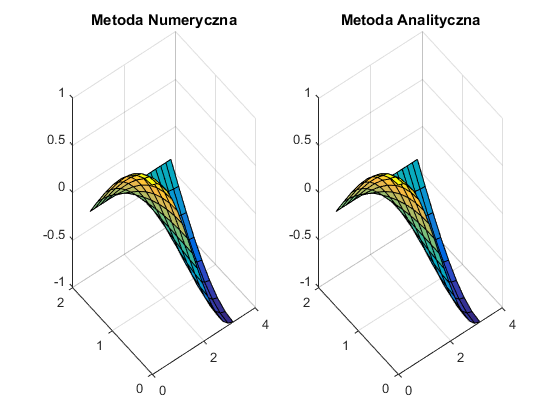
\includegraphics[width=0.8\textwidth]{Lab6/charts/jacobi/zad2/15.png}
	\end{center}
\end{figure}

Liczba wykonanych iteracji $ = 138 $

Czas wykonywania algorytmu $ = 0.179 s$

Dla n = 35:

\begin{figure}[!ht]
	\begin{center}
		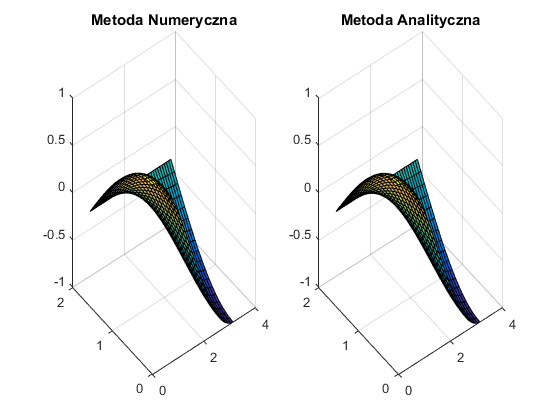
\includegraphics[width=0.8\textwidth]{Lab6/charts/jacobi/zad2/35.png}
	\end{center}
\end{figure}

Liczba wykonanych iteracji $ = 529 $

Czas wykonywania algorytmu $ = 0.294 s$



Dla n = 55:

\begin{figure}[!ht]
	\begin{center}
		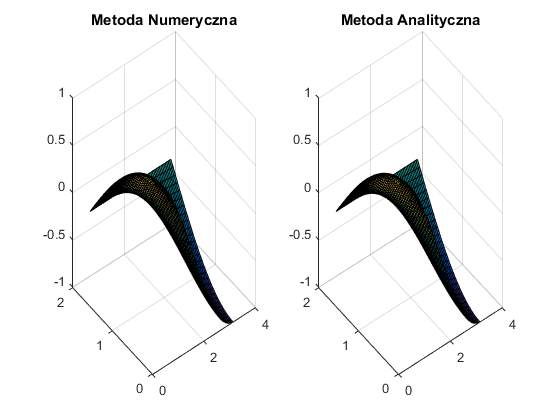
\includegraphics[width=0.8\textwidth]{Lab6/charts/jacobi/zad2/55.png}
	\end{center}
\end{figure}

Liczba wykonanych iteracji $ = 1058 $

Czas wykonywania algorytmu $ = 0.753 s$

\newpage
\subsection{Metoda Gaussa - Seidela	}

Jest to dowolona modyfikacja metody Jacobiego, a wprowadzana zmiana niemal dwukrotnie przyspiesza tempo zbieżności.

W metodzie tej wartości przybliżone rozwiązania numerycznego są poprawiane w węzłach siatki zgodnie z ustalonym przez cały proces iteraycjny porządkiem.

Dowolne pierwsze przybliżenie (poprawione):

$$u_{i,j}^{(n+1)} = \frac{1}{4}(u_{i+1,j}^{(n)} + u_{i-1,j}^{(n+1)} + u_{i,j+1}^{(n)} + u_{i,j-1}^{(n+1)}) - \frac{1}{4}h^2f_{i,j}$$

Schemat ten jest pozornie niejawny, ale w rzeczywistości uwzględnia on w kroku $n+1$ poprawkę wcześniej już obliczoną.
\newpage
\subsubsection{Algorytm}

a)

\begin{Shaded}
\begin{Highlighting}[]
\CommentTok{%metoda Gaussa - Seidela}
\FunctionTok{clc}\NormalTok{, }\FunctionTok{clear} \FunctionTok{all}\NormalTok{; }\FunctionTok{tic}
\CommentTok{%funkcja}
\NormalTok{F = @(x,y) }\FloatTok{0}\NormalTok{;}
\CommentTok{%rozwiązanie analityczne}
\NormalTok{G = @(x,y) }\FunctionTok{log}\NormalTok{(x.^}\FloatTok{2}\NormalTok{+y.^}\FloatTok{2}\NormalTok{);}
\CommentTok{%przedział omega}
\NormalTok{xa=}\FloatTok{1}\NormalTok{; xb=}\FloatTok{2}\NormalTok{; yc=}\FloatTok{0}\NormalTok{; yd=}\FloatTok{1}\NormalTok{;}
\CommentTok{%warunki brzegowe}
\NormalTok{war1 = @(x) }\FloatTok{2}\NormalTok{*}\FunctionTok{log}\NormalTok{(x);}
\NormalTok{war2 = @(y) }\FunctionTok{log}\NormalTok{(y.^}\FloatTok{2}\NormalTok{+}\FloatTok{4}\NormalTok{);}
\NormalTok{war3 = @(x) }\FunctionTok{log}\NormalTok{(x.^}\FloatTok{2}\NormalTok{+}\FloatTok{1}\NormalTok{);}
\NormalTok{war4 = @(y) }\FunctionTok{log}\NormalTok{(y.^}\FloatTok{2}\NormalTok{+}\FloatTok{1}\NormalTok{);}
\CommentTok{%siatka}
\NormalTok{n=}\FloatTok{50}\NormalTok{; m=n;}
\NormalTok{h=(xb-xa)/(n-}\FloatTok{1}\NormalTok{);}
\NormalTok{x=}\FunctionTok{linspace}\NormalTok{(xa,xb,n+}\FloatTok{2}\NormalTok{);}
\NormalTok{y=}\FunctionTok{linspace}\NormalTok{(yc,yd,m+}\FloatTok{2}\NormalTok{);}
\NormalTok{tol=}\FloatTok{1e-4}\NormalTok{; }\FunctionTok{error}\NormalTok{ = }\FloatTok{10}\NormalTok{; licznik=}\FloatTok{0}\NormalTok{; }
\CommentTok{%tworzenie macierzy}
\NormalTok{M0=}\FunctionTok{zeros}\NormalTok{(m,n)+}\FloatTok{1}\NormalTok{;}
\NormalTok{M1(}\FloatTok{1}\NormalTok{:n+}\FloatTok{2}\NormalTok{) = war1(x);}
\NormalTok{M2(}\FloatTok{1}\NormalTok{:m) = war2(y(}\FloatTok{2}\NormalTok{:}\FunctionTok{length}\NormalTok{(y)-}\FloatTok{1}\NormalTok{));}
\NormalTok{M3(}\FloatTok{1}\NormalTok{:n+}\FloatTok{2}\NormalTok{) = war3(x);}
\NormalTok{M4(}\FloatTok{1}\NormalTok{:m) = war4(y(}\FloatTok{2}\NormalTok{:}\FunctionTok{length}\NormalTok{(y)-}\FloatTok{1}\NormalTok{));}
\NormalTok{M0=[M4', M0, M2']; M0=[M1;M0;M3]; M=M0;}
\NormalTok{for }\BaseNTok{i}\NormalTok{=}\FloatTok{1}\NormalTok{:m+}\FloatTok{2}
\NormalTok{    for }\BaseNTok{j}\NormalTok{=}\FloatTok{1}\NormalTok{:n+}\FloatTok{2}
\NormalTok{        g(}\BaseNTok{i}\NormalTok{,}\BaseNTok{j}\NormalTok{) = G(x(}\BaseNTok{j}\NormalTok{),y(}\BaseNTok{i}\NormalTok{));}
\NormalTok{    end}
\NormalTok{end}
\NormalTok{while }\FunctionTok{error}\NormalTok{>tol}
\NormalTok{    for }\BaseNTok{i}\NormalTok{=}\FloatTok{2}\NormalTok{:m+}\FloatTok{1}
\NormalTok{        for }\BaseNTok{j}\NormalTok{=}\FloatTok{2}\NormalTok{:n+}\FloatTok{1}
\NormalTok{            M(}\BaseNTok{i}\NormalTok{,}\BaseNTok{j}\NormalTok{) =}\FloatTok{0.25}\NormalTok{*(M(}\BaseNTok{i}\NormalTok{+}\FloatTok{1}\NormalTok{,}\BaseNTok{j}\NormalTok{)+M(}\BaseNTok{i}\NormalTok{-}\FloatTok{1}\NormalTok{,}\BaseNTok{j}\NormalTok{)+M(}\BaseNTok{i}\NormalTok{,}\BaseNTok{j}\NormalTok{+}\FloatTok{1}\NormalTok{)+M(}\BaseNTok{i}\NormalTok{,}\BaseNTok{j}\NormalTok{-}\FloatTok{1}\NormalTok{))-}\FloatTok{0.25}\NormalTok{*h^}\FloatTok{2}\NormalTok{*F(x(}\BaseNTok{j}\NormalTok{),y(}\BaseNTok{i}\NormalTok{));}
\NormalTok{        end}
\NormalTok{    end}
    \FunctionTok{error}\NormalTok{=}\FunctionTok{max}\NormalTok{(}\FunctionTok{max}\NormalTok{(}\FunctionTok{abs}\NormalTok{(M0-M)));}
\NormalTok{    M0=M; licznik = licznik+}\FloatTok{1}\NormalTok{;}
\NormalTok{end}
\CommentTok{%wykresy}
\NormalTok{[X,Y] = }\FunctionTok{meshgrid}\NormalTok{(x,y);}
\FunctionTok{subplot}\NormalTok{(}\FloatTok{1}\NormalTok{,}\FloatTok{2}\NormalTok{,}\FloatTok{1}\NormalTok{)}
\FunctionTok{surf}\NormalTok{(X,Y,M0)}
\FunctionTok{title}\NormalTok{(}\StringTok{'Metoda Numeryczna'}\NormalTok{)}
\FunctionTok{subplot}\NormalTok{(}\FloatTok{1}\NormalTok{,}\FloatTok{2}\NormalTok{,}\FloatTok{2}\NormalTok{)}
\FunctionTok{surf}\NormalTok{(X,Y,(G(X,Y)))}
\FunctionTok{title}\NormalTok{(}\StringTok{'Metoda Analityczna'}\NormalTok{)}
\NormalTok{licznik; }\FunctionTok{toc}
\end{Highlighting}
\end{Shaded}
\newpage
b)

\begin{Shaded}
\begin{Highlighting}[]
\CommentTok{%metoda Gaussa - Seidela}
\FunctionTok{clc}\NormalTok{, }\FunctionTok{clear} \FunctionTok{all}\NormalTok{; }\FunctionTok{tic}
\CommentTok{%funkcja}
\NormalTok{F = @(x,y) -}\FunctionTok{cos}\NormalTok{(x+y)-}\FunctionTok{cos}\NormalTok{(x-y);}
\CommentTok{%rozwiązanie analityczne}
\NormalTok{G = @(x,y) }\FunctionTok{cos}\NormalTok{(x).*}\FunctionTok{cos}\NormalTok{(y);}
\CommentTok{%przedział omega}
\NormalTok{xa=}\FloatTok{0}\NormalTok{; xb=}\BaseNTok{pi}\NormalTok{; yc=}\FloatTok{0}\NormalTok{; yd=}\BaseNTok{pi}\NormalTok{/}\FloatTok{2}\NormalTok{;}
\CommentTok{%warunki brzegowe}
\NormalTok{war1 = @(x) }\FunctionTok{cos}\NormalTok{(x);}
\NormalTok{war2 = @(y) -}\FunctionTok{cos}\NormalTok{(y);}
\NormalTok{war3 = @(x) }\FloatTok{0}\NormalTok{;}
\NormalTok{war4 = @(y) }\FunctionTok{cos}\NormalTok{(y);}
\CommentTok{%siatka}
\NormalTok{n=}\FloatTok{50}\NormalTok{; m=(yd-yc)/(xb-xa)*(n+}\FloatTok{1}\NormalTok{)-}\FloatTok{1}\NormalTok{;}
\NormalTok{h=(xb-xa)/(n-}\FloatTok{1}\NormalTok{);}
\NormalTok{x=}\FunctionTok{linspace}\NormalTok{(xa,xb,n+}\FloatTok{2}\NormalTok{);}
\NormalTok{y=}\FunctionTok{linspace}\NormalTok{(yc,yd,m+}\FloatTok{2}\NormalTok{);}
\NormalTok{tol=}\FloatTok{1e-4}\NormalTok{; }\FunctionTok{error}\NormalTok{ = }\FloatTok{10}\NormalTok{; licznik=}\FloatTok{0}\NormalTok{; }
\CommentTok{%tworzenie macierzy}
\NormalTok{M0=}\FunctionTok{zeros}\NormalTok{(m,n)+}\FloatTok{1}\NormalTok{;}
\NormalTok{M1(}\FloatTok{1}\NormalTok{:n+}\FloatTok{2}\NormalTok{) = war1(x);}
\NormalTok{M2(}\FloatTok{1}\NormalTok{:m) = war2(y(}\FloatTok{2}\NormalTok{:}\FunctionTok{length}\NormalTok{(y)-}\FloatTok{1}\NormalTok{));}
\NormalTok{M3(}\FloatTok{1}\NormalTok{:n+}\FloatTok{2}\NormalTok{) = war3(x);}
\NormalTok{M4(}\FloatTok{1}\NormalTok{:m) = war4(y(}\FloatTok{2}\NormalTok{:}\FunctionTok{length}\NormalTok{(y)-}\FloatTok{1}\NormalTok{));}
\NormalTok{M0=[M4', M0, M2']; M0=[M1;M0;M3]; M=M0;}
\NormalTok{for }\BaseNTok{i}\NormalTok{=}\FloatTok{1}\NormalTok{:m+}\FloatTok{2}
\NormalTok{    for }\BaseNTok{j}\NormalTok{=}\FloatTok{1}\NormalTok{:n+}\FloatTok{2}
\NormalTok{        g(}\BaseNTok{i}\NormalTok{,}\BaseNTok{j}\NormalTok{) = G(x(}\BaseNTok{j}\NormalTok{),y(}\BaseNTok{i}\NormalTok{));}
\NormalTok{    end}
\NormalTok{end}
\NormalTok{while }\FunctionTok{error}\NormalTok{>tol}
\NormalTok{    for }\BaseNTok{i}\NormalTok{=}\FloatTok{2}\NormalTok{:m+}\FloatTok{1}
\NormalTok{        for }\BaseNTok{j}\NormalTok{=}\FloatTok{2}\NormalTok{:n+}\FloatTok{1}
\NormalTok{            M(}\BaseNTok{i}\NormalTok{,}\BaseNTok{j}\NormalTok{) =}\FloatTok{0.25}\NormalTok{*(M(}\BaseNTok{i}\NormalTok{+}\FloatTok{1}\NormalTok{,}\BaseNTok{j}\NormalTok{)+M(}\BaseNTok{i}\NormalTok{-}\FloatTok{1}\NormalTok{,}\BaseNTok{j}\NormalTok{)+M(}\BaseNTok{i}\NormalTok{,}\BaseNTok{j}\NormalTok{+}\FloatTok{1}\NormalTok{)+M(}\BaseNTok{i}\NormalTok{,}\BaseNTok{j}\NormalTok{-}\FloatTok{1}\NormalTok{))-}\FloatTok{0.25}\NormalTok{*h^}\FloatTok{2}\NormalTok{*F(x(}\BaseNTok{j}\NormalTok{),y(}\BaseNTok{i}\NormalTok{));}
\NormalTok{        end}
\NormalTok{    end}
    \FunctionTok{error}\NormalTok{=}\FunctionTok{max}\NormalTok{(}\FunctionTok{max}\NormalTok{(}\FunctionTok{abs}\NormalTok{(M0-M)));}
\NormalTok{    M0=M; licznik = licznik+}\FloatTok{1}\NormalTok{;}
\NormalTok{end}
\CommentTok{%wykresy}
\NormalTok{[X,Y] = }\FunctionTok{meshgrid}\NormalTok{(x,y);}
\FunctionTok{subplot}\NormalTok{(}\FloatTok{1}\NormalTok{,}\FloatTok{2}\NormalTok{,}\FloatTok{1}\NormalTok{)}
\FunctionTok{surf}\NormalTok{(X,Y,M0)}
\FunctionTok{title}\NormalTok{(}\StringTok{'Metoda Numeryczna'}\NormalTok{)}
\FunctionTok{subplot}\NormalTok{(}\FloatTok{1}\NormalTok{,}\FloatTok{2}\NormalTok{,}\FloatTok{2}\NormalTok{)}
\FunctionTok{surf}\NormalTok{(X,Y,(G(X,Y)))}
\FunctionTok{title}\NormalTok{(}\StringTok{'Metoda Analityczna'}\NormalTok{)}
\NormalTok{licznik; }\FunctionTok{toc}
\end{Highlighting}
\end{Shaded}
\newpage
\subsubsection{Wykresy}

a)

Dla n = 5:

\begin{figure}[!ht]
	\begin{center}
		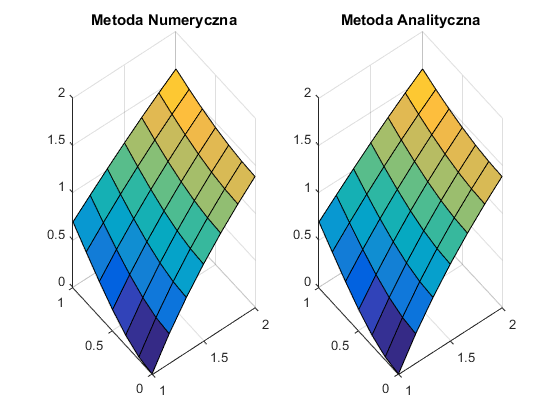
\includegraphics[width=0.78\textwidth]{Lab6/charts/gs/zad1/5.png}
	\end{center}
\end{figure}

Liczba wykonanych iteracji $ = 21 $

Czas wykonywania algorytmu $ = 0.167 s$

Dla n = 15:

\begin{figure}[!ht]
	\begin{center}
		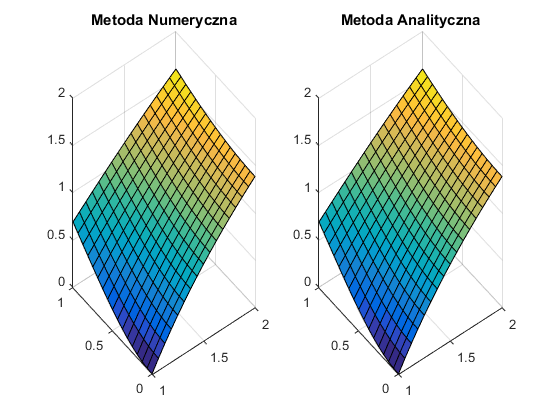
\includegraphics[width=0.78\textwidth]{Lab6/charts/gs/zad1/15.png}
	\end{center}
\end{figure}
Liczba wykonanych iteracji $ = 75 $

Czas wykonywania algorytmu $ = 0.181 s$

\newpage
Dla n = 30:

\begin{figure}[!ht]
	\begin{center}
		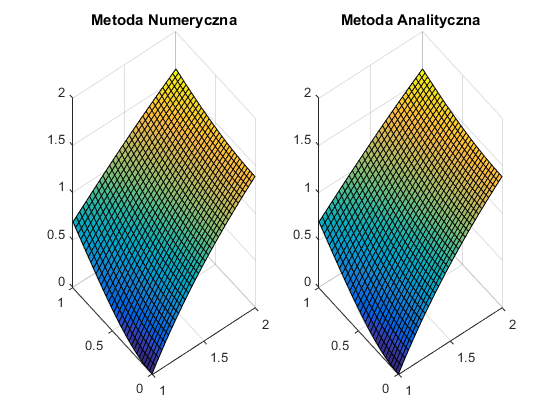
\includegraphics[width=0.8\textwidth]{Lab6/charts/gs/zad1/30.png}
	\end{center}
\end{figure}

Liczba wykonanych iteracji $ = 232 $

Czas wykonywania algorytmu $ = 0.241 s$

Dla n = 50:

\begin{figure}[!ht]
	\begin{center}
		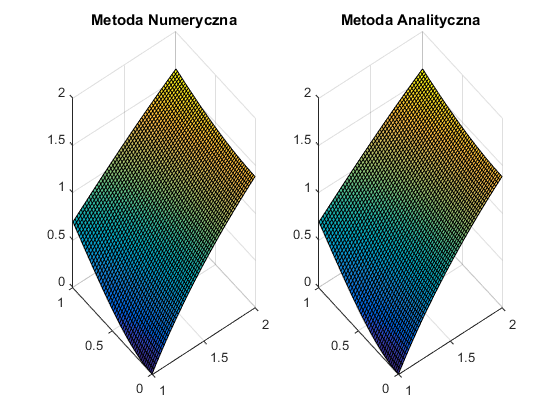
\includegraphics[width=0.8\textwidth]{Lab6/charts/gs/zad1/50.png}
	\end{center}
\end{figure}

Liczba wykonanych iteracji $ = 485 $

Czas wykonywania algorytmu $ = 0.548 s$
\newpage
b)

Dla n = 5:

\begin{figure}[!ht]
	\begin{center}
		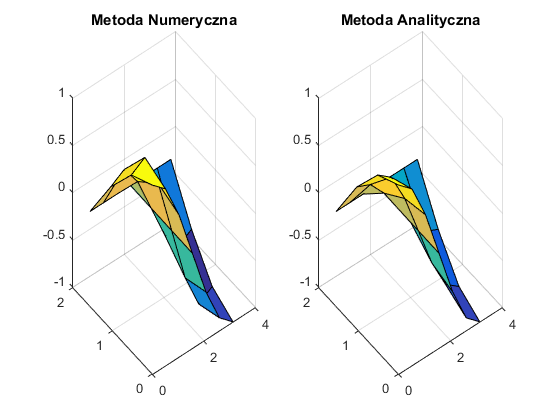
\includegraphics[width=0.8\textwidth]{Lab6/charts/gs/zad2/5.png}
	\end{center}
\end{figure}

Liczba wykonanych iteracji $ = 14 $

Czas wykonywania algorytmu $ = 0.177 s$

Dla n = 15:

\begin{figure}[!ht]
	\begin{center}
		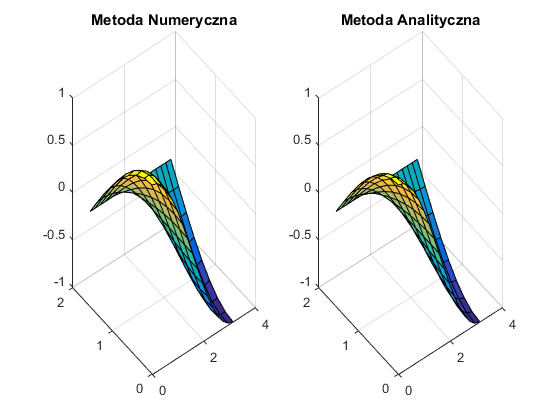
\includegraphics[width=0.8\textwidth]{Lab6/charts/gs/zad2/15.png}
	\end{center}
\end{figure}

Liczba wykonanych iteracji $ = 78 $

Czas wykonywania algorytmu $ = 0.175 s$
\newpage
Dla n = 35:

\begin{figure}[!ht]
	\begin{center}
		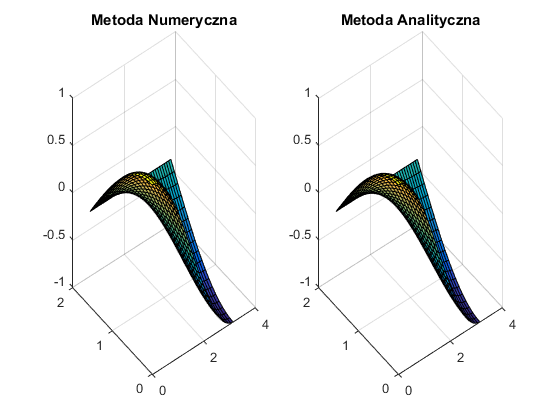
\includegraphics[width=0.8\textwidth]{Lab6/charts/gs/zad2/35.png}
	\end{center}
\end{figure}

Liczba wykonanych iteracji $ = 304 $

Czas wykonywania algorytmu $ = 0.242 s$

Dla n = 55:

\begin{figure}[!ht]
	\begin{center}
		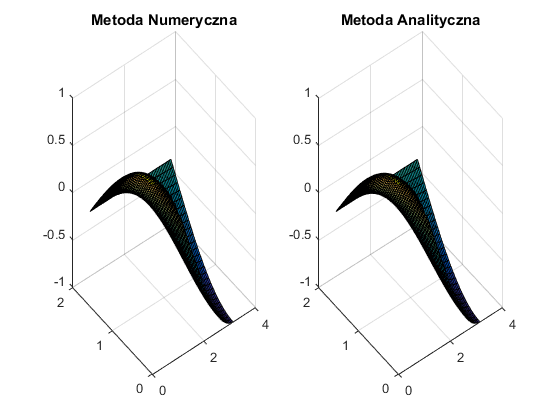
\includegraphics[width=0.8\textwidth]{Lab6/charts/gs/zad2/55.png}
	\end{center}
\end{figure}

Liczba wykonanych iteracji $ = 621 $

Czas wykonywania algorytmu $ = 0.511 s$
\newpage
\subsection{Metoda nadrelaksacji Younge'a}

Rozważmy modyfikację metody Gaussa $-$ Seidela.

$$u_{i,j}^{(n+1)} = \frac{1}{4}\omega(u_{i+1,j}^{(n)} + u_{i-1,j}^{(n+1)} + u_{i,j+1}^{(n)} + u_{i,j-1}^{(n+1)}) + (1-\omega)u^n_{i,j} - \frac{1}{4}h^2f_{i,j}$$

, gdzie $\omega \hspace{0.1cm} -$ parametr relaksacji

Zauważmy, gdy $\omega = 1$, otrzymujemy metodę Gaussa $-$ Seidela. 

Właściwy wybór parametru relaksacji pozwala na znaczące przyspieszenie zbieżności metody.

Young udowodnił, że wartość optymalna $\omega$ dana jest następującą zależnością:

$$\omega_{opt}=1+\dfrac{\lambda}{(1+\sqrt{1-\lambda})^2}$$

$$\lambda = \dfrac{1}{4}\Big(\cos\Big(\dfrac{\pi}{N}\Big) + \cos\Big(\dfrac{\pi}{M}\Big)\Big)^2$$

, gdzie: M oraz N to liczba elementów, na które podzielono boki

W przypadku innej geometrii niż prostokątna, dla równań Laplace'a i Poissona, $\lambda$ można obliczyć korzystając z tej zależności biorąc wymiar największego prostokąta, który zawiera ten obszar.

Tak wyznaczony parametr relaksacji będzie wyższy niż optymalny, lecz Young udowodnił, że taki nadmiarowy współczynnik, nie zmniejsza znacząco szybkości zbieżności tej metody.
\newpage
\subsubsection{Algorytm}

a)

\begin{Shaded}
\begin{Highlighting}[]
\CommentTok{%metoda Younga}
\FunctionTok{clc}\NormalTok{, }\FunctionTok{clear} \FunctionTok{all}\NormalTok{; }\FunctionTok{tic}
\CommentTok{%funkcja}
\NormalTok{F = @(x,y) }\FloatTok{0}\NormalTok{;}
\CommentTok{%rozwiązanie analityczne}
\NormalTok{G = @(x,y) }\FunctionTok{log}\NormalTok{(x.^}\FloatTok{2}\NormalTok{+y.^}\FloatTok{2}\NormalTok{);}
\CommentTok{%przedział omega}
\NormalTok{xa=}\FloatTok{1}\NormalTok{; xb=}\FloatTok{2}\NormalTok{; yc=}\FloatTok{0}\NormalTok{; yd=}\FloatTok{1}\NormalTok{;}
\CommentTok{%warunki brzegowe}
\NormalTok{war1 = @(x) }\FloatTok{2}\NormalTok{*}\FunctionTok{log}\NormalTok{(x);}
\NormalTok{war2 = @(y) }\FunctionTok{log}\NormalTok{(y.^}\FloatTok{2}\NormalTok{+}\FloatTok{4}\NormalTok{);}
\NormalTok{war3 = @(x) }\FunctionTok{log}\NormalTok{(x.^}\FloatTok{2}\NormalTok{+}\FloatTok{1}\NormalTok{);}
\NormalTok{war4 = @(y) }\FunctionTok{log}\NormalTok{(y.^}\FloatTok{2}\NormalTok{+}\FloatTok{1}\NormalTok{);}
\CommentTok{%siatka}
\NormalTok{n=}\FloatTok{35}\NormalTok{; m=n;}
\NormalTok{lambda = }\FloatTok{0.25}\NormalTok{*(}\FunctionTok{cos}\NormalTok{(}\BaseNTok{pi}\NormalTok{/n)+}\FunctionTok{cos}\NormalTok{(}\BaseNTok{pi}\NormalTok{/m))^}\FloatTok{2}\NormalTok{;}
\NormalTok{omega = }\FloatTok{1}\NormalTok{+(lambda/(}\FloatTok{1}\NormalTok{+}\FunctionTok{sqrt}\NormalTok{(}\FloatTok{1}\NormalTok{-lambda))^}\FloatTok{2}\NormalTok{);}
\NormalTok{h=(xb-xa)/(n-}\FloatTok{1}\NormalTok{); x=}\FunctionTok{linspace}\NormalTok{(xa,xb,n+}\FloatTok{2}\NormalTok{); y=}\FunctionTok{linspace}\NormalTok{(yc,yd,m+}\FloatTok{2}\NormalTok{);}
\NormalTok{tol=}\FloatTok{1e-2}\NormalTok{; }\FunctionTok{error}\NormalTok{ = }\FloatTok{10}\NormalTok{; licznik=}\FloatTok{0}\NormalTok{; }
\CommentTok{%tworzenie macierzy}
\NormalTok{M0=}\FunctionTok{zeros}\NormalTok{(m,n)+}\FloatTok{1}\NormalTok{;}
\NormalTok{M1(}\FloatTok{1}\NormalTok{:n+}\FloatTok{2}\NormalTok{) = war1(x);}
\NormalTok{M2(}\FloatTok{1}\NormalTok{:m) = war2(y(}\FloatTok{2}\NormalTok{:}\FunctionTok{length}\NormalTok{(y)-}\FloatTok{1}\NormalTok{));}
\NormalTok{M3(}\FloatTok{1}\NormalTok{:n+}\FloatTok{2}\NormalTok{) = war3(x);}
\NormalTok{M4(}\FloatTok{1}\NormalTok{:m) = war4(y(}\FloatTok{2}\NormalTok{:}\FunctionTok{length}\NormalTok{(y)-}\FloatTok{1}\NormalTok{));}
\NormalTok{M0=[M4', M0, M2']; M0=[M1;M0;M3]; M=M0;}
\NormalTok{for }\BaseNTok{i}\NormalTok{=}\FloatTok{1}\NormalTok{:m+}\FloatTok{2}
\NormalTok{    for }\BaseNTok{j}\NormalTok{=}\FloatTok{1}\NormalTok{:n+}\FloatTok{2}
\NormalTok{        g(}\BaseNTok{i}\NormalTok{,}\BaseNTok{j}\NormalTok{) = G(x(}\BaseNTok{j}\NormalTok{),y(}\BaseNTok{i}\NormalTok{));}
\NormalTok{    end}
\NormalTok{end}
\NormalTok{while }\FunctionTok{error}\NormalTok{>tol}
\NormalTok{    for }\BaseNTok{i}\NormalTok{=}\FloatTok{2}\NormalTok{:m+}\FloatTok{1}
\NormalTok{        for }\BaseNTok{j}\NormalTok{=}\FloatTok{2}\NormalTok{:n+}\FloatTok{1}
\NormalTok{            M(}\BaseNTok{i}\NormalTok{,}\BaseNTok{j}\NormalTok{) =}\FloatTok{0.25}\NormalTok{*omega*(M(}\BaseNTok{i}\NormalTok{+}\FloatTok{1}\NormalTok{,}\BaseNTok{j}\NormalTok{)+M(}\BaseNTok{i}\NormalTok{-}\FloatTok{1}\NormalTok{,}\BaseNTok{j}\NormalTok{)\textbackslash{}+M(}\BaseNTok{i}\NormalTok{,}\BaseNTok{j}\NormalTok{+}\FloatTok{1}\NormalTok{)+M(}\BaseNTok{i}\NormalTok{,}\BaseNTok{j}\NormalTok{-}\FloatTok{1}\NormalTok{))\textbackslash{}}
\NormalTok{            +(}\FloatTok{1}\NormalTok{-omega)*M(}\BaseNTok{i}\NormalTok{,}\BaseNTok{j}\NormalTok{)-}\FloatTok{0.25}\NormalTok{*h^}\FloatTok{2}\NormalTok{*F(x(}\BaseNTok{j}\NormalTok{),y(}\BaseNTok{i}\NormalTok{));}
\NormalTok{        end}
\NormalTok{    end}
    \FunctionTok{error}\NormalTok{=}\FunctionTok{max}\NormalTok{(}\FunctionTok{max}\NormalTok{(}\FunctionTok{abs}\NormalTok{(M0-M)));}
\NormalTok{    M0=M; licznik = licznik+}\FloatTok{1}\NormalTok{;}
\NormalTok{end}
\CommentTok{%wykresy}
\NormalTok{[X,Y] = }\FunctionTok{meshgrid}\NormalTok{(x,y);}
\FunctionTok{subplot}\NormalTok{(}\FloatTok{1}\NormalTok{,}\FloatTok{2}\NormalTok{,}\FloatTok{1}\NormalTok{)}
\FunctionTok{surf}\NormalTok{(X,Y,M0)}
\FunctionTok{title}\NormalTok{(}\StringTok{'Metoda Numeryczna'}\NormalTok{)}
\FunctionTok{subplot}\NormalTok{(}\FloatTok{1}\NormalTok{,}\FloatTok{2}\NormalTok{,}\FloatTok{2}\NormalTok{)}
\FunctionTok{surf}\NormalTok{(X,Y,(G(X,Y)))}
\FunctionTok{title}\NormalTok{(}\StringTok{'Metoda Analityczna'}\NormalTok{)}
\NormalTok{licznik; }\FunctionTok{toc}
\end{Highlighting}
\end{Shaded}
\newpage
b)

\begin{Shaded}
\begin{Highlighting}[]
\CommentTok{%metoda Younga}
\FunctionTok{clc}\NormalTok{, }\FunctionTok{clear} \FunctionTok{all}\NormalTok{; }\FunctionTok{tic}
\CommentTok{%funkcja}
\NormalTok{F = @(x,y) -}\FunctionTok{cos}\NormalTok{(x+y)-}\FunctionTok{cos}\NormalTok{(x-y);}
\CommentTok{%rozwiązanie analityczne}
\NormalTok{G = @(x,y) }\FunctionTok{cos}\NormalTok{(x).*}\FunctionTok{cos}\NormalTok{(y);}
\CommentTok{%przedział omega}
\NormalTok{xa=}\FloatTok{0}\NormalTok{; xb=}\BaseNTok{pi}\NormalTok{; yc=}\FloatTok{0}\NormalTok{; yd=}\BaseNTok{pi}\NormalTok{/}\FloatTok{2}\NormalTok{;}
\CommentTok{%warunki brzegowe}
\NormalTok{war1 = @(x) }\FunctionTok{cos}\NormalTok{(x);}
\NormalTok{war2 = @(y) -}\FunctionTok{cos}\NormalTok{(y);}
\NormalTok{war3 = @(x) }\FloatTok{0}\NormalTok{;}
\NormalTok{war4 = @(y) }\FunctionTok{cos}\NormalTok{(y);}
\CommentTok{%siatka}
\NormalTok{n=}\FloatTok{55}\NormalTok{; m=(yd-yc)/(xb-xa)*(n+}\FloatTok{1}\NormalTok{)-}\FloatTok{1}\NormalTok{;}
\NormalTok{lambda = }\FloatTok{0.25}\NormalTok{*(}\FunctionTok{cos}\NormalTok{(}\BaseNTok{pi}\NormalTok{/n)+}\FunctionTok{cos}\NormalTok{(}\BaseNTok{pi}\NormalTok{/m))^}\FloatTok{2}\NormalTok{;}
\NormalTok{omega = }\FloatTok{1}\NormalTok{+(lambda/(}\FloatTok{1}\NormalTok{+}\FunctionTok{sqrt}\NormalTok{(}\FloatTok{1}\NormalTok{-lambda))^}\FloatTok{2}\NormalTok{);}
\NormalTok{h=(xb-xa)/(n+}\FloatTok{1}\NormalTok{); x=}\FunctionTok{linspace}\NormalTok{(xa,xb,n+}\FloatTok{2}\NormalTok{); y=}\FunctionTok{linspace}\NormalTok{(yc,yd,m+}\FloatTok{2}\NormalTok{);}
\NormalTok{tol=}\FloatTok{1e-4}\NormalTok{; }\FunctionTok{error}\NormalTok{ = }\FloatTok{10}\NormalTok{; licznik=}\FloatTok{0}\NormalTok{; }
\CommentTok{%tworzenie macierzy}
\NormalTok{M0=}\FunctionTok{zeros}\NormalTok{(m,n)+}\FloatTok{1}\NormalTok{;}
\NormalTok{M1(}\FloatTok{1}\NormalTok{:n+}\FloatTok{2}\NormalTok{) = war1(x);}
\NormalTok{M2(}\FloatTok{1}\NormalTok{:m) = war2(y(}\FloatTok{2}\NormalTok{:}\FunctionTok{length}\NormalTok{(y)-}\FloatTok{1}\NormalTok{));}
\NormalTok{M3(}\FloatTok{1}\NormalTok{:n+}\FloatTok{2}\NormalTok{) = war3(x);}
\NormalTok{M4(}\FloatTok{1}\NormalTok{:m) = war4(y(}\FloatTok{2}\NormalTok{:}\FunctionTok{length}\NormalTok{(y)-}\FloatTok{1}\NormalTok{));}
\NormalTok{M0=[M4', M0, M2']; M0=[M1;M0;M3]; M=M0;}
\NormalTok{for }\BaseNTok{i}\NormalTok{=}\FloatTok{1}\NormalTok{:m+}\FloatTok{2}
\NormalTok{    for }\BaseNTok{j}\NormalTok{=}\FloatTok{1}\NormalTok{:n+}\FloatTok{2}
\NormalTok{        g(}\BaseNTok{i}\NormalTok{,}\BaseNTok{j}\NormalTok{) = G(x(}\BaseNTok{j}\NormalTok{),y(}\BaseNTok{i}\NormalTok{));}
\NormalTok{    end}
\NormalTok{end}
\NormalTok{while }\FunctionTok{error}\NormalTok{>tol}
\NormalTok{    for }\BaseNTok{i}\NormalTok{=}\FloatTok{2}\NormalTok{:m+}\FloatTok{1}
\NormalTok{        for }\BaseNTok{j}\NormalTok{=}\FloatTok{2}\NormalTok{:n+}\FloatTok{1}
\NormalTok{            M(}\BaseNTok{i}\NormalTok{,}\BaseNTok{j}\NormalTok{) =}\FloatTok{0.25}\NormalTok{*omega*(M(}\BaseNTok{i}\NormalTok{+}\FloatTok{1}\NormalTok{,}\BaseNTok{j}\NormalTok{)+M(}\BaseNTok{i}\NormalTok{-}\FloatTok{1}\NormalTok{,}\BaseNTok{j}\NormalTok{)+M(}\BaseNTok{i}\NormalTok{,}\BaseNTok{j}\NormalTok{+}\FloatTok{1}\NormalTok{)+M(}\BaseNTok{i}\NormalTok{,}\BaseNTok{j}\NormalTok{-}\FloatTok{1}\NormalTok{))\textbackslash{}}
\NormalTok{            +(}\FloatTok{1}\NormalTok{-omega)*M(}\BaseNTok{i}\NormalTok{,}\BaseNTok{j}\NormalTok{)-}\FloatTok{0.25}\NormalTok{*h^}\FloatTok{2}\NormalTok{*F(x(}\BaseNTok{j}\NormalTok{),y(}\BaseNTok{i}\NormalTok{));}
\NormalTok{        end}
\NormalTok{    end}
    \FunctionTok{error}\NormalTok{=}\FunctionTok{max}\NormalTok{(}\FunctionTok{max}\NormalTok{(}\FunctionTok{abs}\NormalTok{(M0-M)));}
\NormalTok{    M0=M; licznik = licznik+}\FloatTok{1}\NormalTok{;}
\NormalTok{end}
\CommentTok{%wykresy}
\NormalTok{[X,Y] = }\FunctionTok{meshgrid}\NormalTok{(x,y);}
\FunctionTok{subplot}\NormalTok{(}\FloatTok{1}\NormalTok{,}\FloatTok{2}\NormalTok{,}\FloatTok{1}\NormalTok{)}
\FunctionTok{surf}\NormalTok{(X,Y,M0)}
\FunctionTok{title}\NormalTok{(}\StringTok{'Metoda Numeryczna'}\NormalTok{)}
\FunctionTok{subplot}\NormalTok{(}\FloatTok{1}\NormalTok{,}\FloatTok{2}\NormalTok{,}\FloatTok{2}\NormalTok{)}
\FunctionTok{surf}\NormalTok{(X,Y,(G(X,Y)))}
\FunctionTok{title}\NormalTok{(}\StringTok{'Metoda Analityczna'}\NormalTok{)}
\NormalTok{licznik; }\FunctionTok{toc}
\end{Highlighting}
\end{Shaded}
\newpage
\subsubsection{Wykresy}

a)

Dla n = 5:

\begin{figure}[!ht]
	\begin{center}
		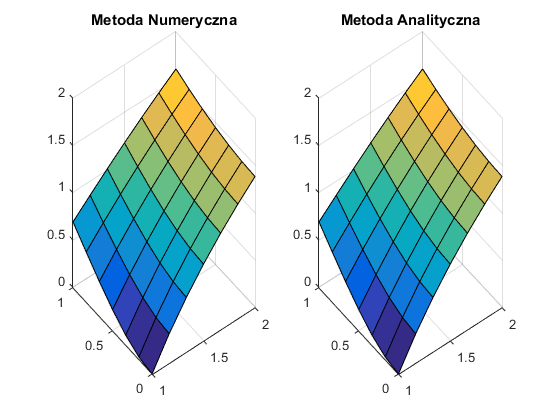
\includegraphics[width=0.78\textwidth]{Lab6/charts/young/zad1/5.png}
	\end{center}
\end{figure}

Liczba wykonanych iteracji $ = 15 $

Czas wykonywania algorytmu $ = 0.183 s$

Dla n = 15:

\begin{figure}[!ht]
	\begin{center}
		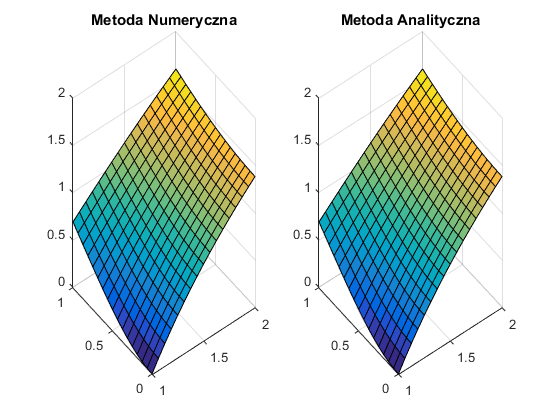
\includegraphics[width=0.78\textwidth]{Lab6/charts/young/zad1/15.png}
	\end{center}
\end{figure}

Liczba wykonanych iteracji $ = 33 $

Czas wykonywania algorytmu $ = 0.181 s$
\newpage
Dla n = 30:

\begin{figure}[!ht]
	\begin{center}
		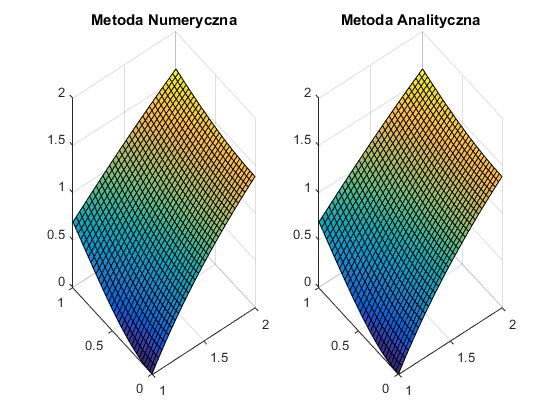
\includegraphics[width=0.8\textwidth]{Lab6/charts/young/zad1/30.png}
	\end{center}
\end{figure}

Liczba wykonanych iteracji $ = 64 $

Czas wykonywania algorytmu $ = 0.197 s$

Dla n = 50:

\begin{figure}[!ht]
	\begin{center}
		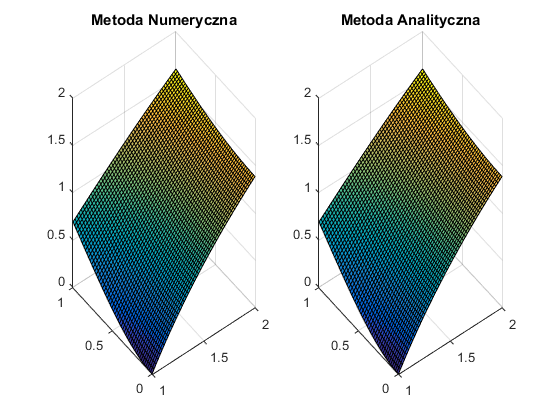
\includegraphics[width=0.8\textwidth]{Lab6/charts/young/zad1/50.png}
	\end{center}
\end{figure}

Liczba wykonanych iteracji $ = 104 $

Czas wykonywania algorytmu $ = 0.269 s$
\newpage
b)

Dla n = 5:

\begin{figure}[!ht]
	\begin{center}
		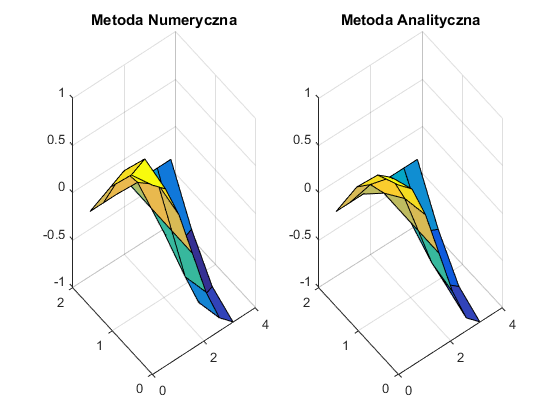
\includegraphics[width=0.8\textwidth]{Lab6/charts/young/zad2/5.png}
	\end{center}
\end{figure}

Liczba wykonanych iteracji $ = 13 $

Czas wykonywania algorytmu $ = 0.176 s$

Dla n = 15:

\begin{figure}[!ht]
	\begin{center}
		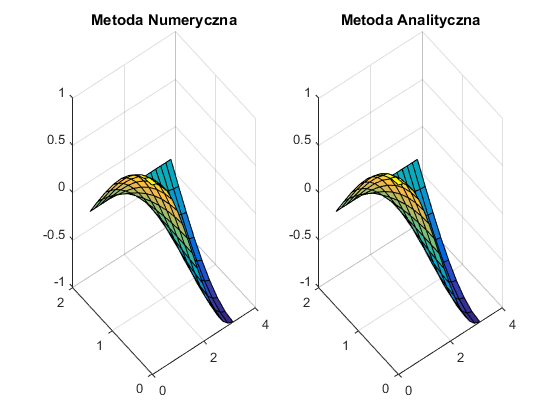
\includegraphics[width=0.8\textwidth]{Lab6/charts/young/zad2/15.png}
	\end{center}
\end{figure}

Liczba wykonanych iteracji $ = 28 $

Czas wykonywania algorytmu $ = 0.180 s$
\newpage
Dla n = 35:

\begin{figure}[!ht]
	\begin{center}
		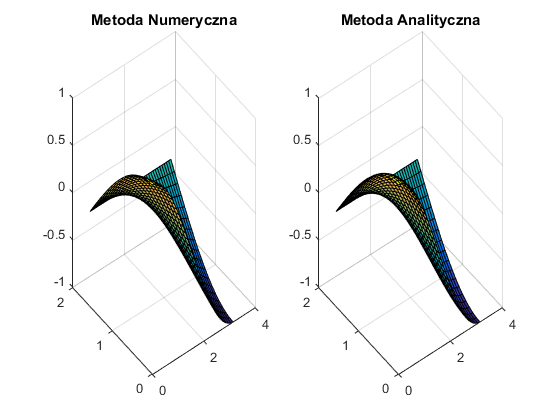
\includegraphics[width=0.8\textwidth]{Lab6/charts/young/zad2/35.png}
	\end{center}
\end{figure}

Liczba wykonanych iteracji $ = 54 $

Czas wykonywania algorytmu $ = 0.192 s$

Dla n = 55:

\begin{figure}[!ht]
	\begin{center}
		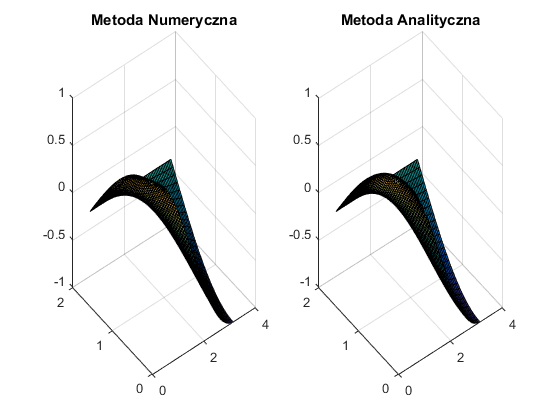
\includegraphics[width=0.8\textwidth]{Lab6/charts/young/zad2/55.png}
	\end{center}
\end{figure}

Liczba wykonanych iteracji $ = 84 $

Czas wykonywania algorytmu $ = 0.227 s$

\newpage
\subsection{Metoda Peacemanna-Rachforda}
Jest to metoda dwupoziomowa niejawna. Charakteryzuje się tym, że kolejne przybliżenia otrzymujemy wykorzystując krok pośredni $n+\frac{1}{2}$.
\\
Przybliżenie w kroku pośrednim $n+\frac{1}{2}$ opisuje poniższe równanie
$$-r u_{i-1,j}^{n+\frac{1}{2}} + (1+2r) u ^{n+\frac{1}{2}}_{i,j} - r u_{i+1,j}^{n+\frac{1}{2}} = u^n_{i,j} + r\left(u^n_{i,j+1} + u^n_{i,j-1} - 2u^n_{i,j} \right)$$
Przybliżenie w kroku $n+1$ otrzymuje się w sposób analogiczny z tą różnicą, że powstały układ równań rozwiązuje się względem kolumn siatki, zamiast względem wierszy.
\\\\
Parametr r w powyższym równaniu definiuje się następująco:\\
Niech $n-1$ oznacza liczbę węzłów wewnętrznych rozważanego wiersza lub kolumny oraz niech $\alpha = sin^2\left(\dfrac{\pi}{2n}\right)$. Wtedy k będzie określone jako najmniejsza dodatnia liczba dla której spełniona jest nierówność
$$\left(\sqrt(2 - 1\right)^{2k} < \alpha$$
, wtedy $$r_i = \alpha^{\dfrac{1+i}{2k}}$$, gdzie $i\in \{1,2,...,k\}$\\
Z tak określonego zbioru parametrów $r_i$ w każdej iteracji wybieramy kolejny parametr w sposób cykliczny.
\newpage
\subsubsection{Algorytm}
Poniżej został przedstawiony algorytm rozwiązania powyższych równań eliptycznych z danymi wejściowymi z podpunktu a).
\begin{Shaded}
\begin{Highlighting}[]
\CommentTok{%metoda Peacemanna-Rachforda}
\FunctionTok{tic}\NormalTok{; }\FunctionTok{clc}\NormalTok{; }\FunctionTok{clear} \FunctionTok{all}
\CommentTok{%funkcja}
\NormalTok{F = @(x,y) }\FloatTok{0}\NormalTok{;}
\CommentTok{%rozwiązanie analityczne}
\NormalTok{G = @(x,y) }\FunctionTok{log}\NormalTok{(x.^}\FloatTok{2}\NormalTok{+y.^}\FloatTok{2}\NormalTok{);}
\CommentTok{%przedział omega}
\NormalTok{xa=}\FloatTok{1}\NormalTok{; xb=}\FloatTok{2}\NormalTok{; yc=}\FloatTok{0}\NormalTok{; yd=}\FloatTok{1}\NormalTok{;}
\CommentTok{%warunki brzegowe}
\NormalTok{u1 = @(x) }\FloatTok{2}\NormalTok{*}\FunctionTok{log}\NormalTok{(x);}
\NormalTok{u2 = @(y) }\FunctionTok{log}\NormalTok{(y.^}\FloatTok{2}\NormalTok{+}\FloatTok{4}\NormalTok{);}
\NormalTok{u3 = @(x) }\FunctionTok{log}\NormalTok{(x.^}\FloatTok{2}\NormalTok{+}\FloatTok{1}\NormalTok{);}
\NormalTok{u4 = @(y) }\FunctionTok{log}\NormalTok{(y.^}\FloatTok{2}\NormalTok{+}\FloatTok{1}\NormalTok{);}
\CommentTok{%siatka}
\NormalTok{n=}\FloatTok{50}\NormalTok{; m=n;}
\NormalTok{h=(xb-xa)/(n+}\FloatTok{1}\NormalTok{); k=(yd-yc)/(m+}\FloatTok{1}\NormalTok{);}
\NormalTok{x=[xa:h:xb]; y=[yc:k:yd];}
\NormalTok{tol=}\FloatTok{1e-4}\NormalTok{; }\FunctionTok{error}\NormalTok{ = }\FloatTok{1}\NormalTok{; licznik=}\FloatTok{0}\NormalTok{; }
\CommentTok{%tworzenie macierzy}
\NormalTok{U = }\FunctionTok{zeros}\NormalTok{(m+}\FloatTok{2}\NormalTok{,n+}\FloatTok{2}\NormalTok{);}
\NormalTok{U(}\FloatTok{1}\NormalTok{,:) = u1(x);}
\NormalTok{U(m+}\FloatTok{2}\NormalTok{,:) = u3(x);}
\NormalTok{U(:,}\FloatTok{1}\NormalTok{) = u4(x);}
\NormalTok{U(:,n+}\FloatTok{2}\NormalTok{) = u2(x);}
\NormalTok{Uk=U;}
\NormalTok{if xb-xa > yd-yc mR = n; else mR = m; end}
\NormalTok{R = createR(mR+}\FloatTok{1}\NormalTok{);}
\NormalTok{lR = }\FunctionTok{length}\NormalTok{(R); }
\NormalTok{while }\FunctionTok{error}\NormalTok{>tol}
\NormalTok{      r = R(}\FunctionTok{mod}\NormalTok{(licznik,lR)+}\FloatTok{1}\NormalTok{);}
      \CommentTok{%step n -> n+1/2}
      \FunctionTok{step}\NormalTok{ = }\BaseNTok{true}\NormalTok{; iter = }\FunctionTok{length}\NormalTok{(y);}
\NormalTok{      for }\BaseNTok{i}\NormalTok{=}\FloatTok{2}\NormalTok{:iter-}\FloatTok{1}
\NormalTok{        Uk(}\BaseNTok{i}\NormalTok{, }\FloatTok{2}\NormalTok{:}\FunctionTok{length}\NormalTok{(x)-}\FloatTok{1}\NormalTok{) = doStep(}\BaseNTok{i}\NormalTok{, r, x, y, U, }\FunctionTok{step}\NormalTok{);}
\NormalTok{      end}
\NormalTok{      U = Uk;}
      \CommentTok{%step n+1/2 -> n+1}
      \FunctionTok{step}\NormalTok{ = }\BaseNTok{false}\NormalTok{; iter = }\FunctionTok{length}\NormalTok{(x);}
\NormalTok{      for }\BaseNTok{i}\NormalTok{=}\FloatTok{2}\NormalTok{:iter-}\FloatTok{1}
\NormalTok{        Uk(}\FloatTok{2}\NormalTok{:}\FunctionTok{length}\NormalTok{(y)-}\FloatTok{1}\NormalTok{, }\BaseNTok{i}\NormalTok{) = doStep(}\BaseNTok{i}\NormalTok{, r, x, y, U, }\FunctionTok{step}\NormalTok{);}
\NormalTok{      end}
\NormalTok{      licznik = licznik+}\FloatTok{1}\NormalTok{;}
      \FunctionTok{error}\NormalTok{ = }\FunctionTok{max}\NormalTok{(}\FunctionTok{max}\NormalTok{(}\FunctionTok{abs}\NormalTok{(Uk-U)));}
\NormalTok{      U=Uk;}
\NormalTok{end}
\CommentTok{%wykresy}
\NormalTok{[X,Y] = }\FunctionTok{meshgrid}\NormalTok{(x,y);}
\FunctionTok{subplot}\NormalTok{(}\FloatTok{1}\NormalTok{,}\FloatTok{2}\NormalTok{,}\FloatTok{1}\NormalTok{)}
\FunctionTok{surf}\NormalTok{(X,Y,U)}
\FunctionTok{title}\NormalTok{(}\StringTok{'Metoda Numeryczna'}\NormalTok{)}
\FunctionTok{subplot}\NormalTok{(}\FloatTok{1}\NormalTok{,}\FloatTok{2}\NormalTok{,}\FloatTok{2}\NormalTok{)}
\FunctionTok{surf}\NormalTok{(X,Y,(G(X,Y)))}
\FunctionTok{title}\NormalTok{(}\StringTok{'Metoda Analityczna'}\NormalTok{)}
\NormalTok{licznik; }\FunctionTok{toc}
\end{Highlighting}
\end{Shaded}
\newpage
\textbf{Funkcje pomocnicze:}\\

Funkcja zwracająca wektor parametrów $r_i$.

\begin{Shaded}
\begin{Highlighting}[]
\NormalTok{function [ r ] = createR( n )}
\NormalTok{a = }\FunctionTok{sin}\NormalTok{(}\BaseNTok{pi}\NormalTok{/(}\FloatTok{2}\NormalTok{*n))^}\FloatTok{2}\NormalTok{;}
\NormalTok{k = }\FloatTok{1}\NormalTok{/}\FloatTok{2}\NormalTok{ * }\FunctionTok{log}\NormalTok{(a)/}\FunctionTok{log}\NormalTok{(}\FunctionTok{sqrt}\NormalTok{(}\FloatTok{2}\NormalTok{)-}\FloatTok{1}\NormalTok{);}
\NormalTok{k = }\FunctionTok{floor}\NormalTok{(k)+}\FloatTok{1}\NormalTok{;}
\NormalTok{r = }\FunctionTok{zeros}\NormalTok{(}\FloatTok{1}\NormalTok{,k);}
\NormalTok{for }\BaseNTok{i}\NormalTok{=}\FloatTok{1}\NormalTok{:k}
\NormalTok{    r(}\BaseNTok{i}\NormalTok{) = a^((}\FloatTok{1}\NormalTok{-}\BaseNTok{i}\NormalTok{)/(}\FloatTok{2}\NormalTok{*k));}
\NormalTok{end}
\NormalTok{end}
\end{Highlighting}
\end{Shaded}

Funkcja obliczająca wiersz lub kolumne w zależności od kroku.

\begin{Shaded}
\begin{Highlighting}[]
\NormalTok{function [Uv] = doStep (iter, r, x, y, U, }\FunctionTok{step}\NormalTok{)}
\NormalTok{if }\FunctionTok{step} \CommentTok{%n-step -> n+1/2  }
\NormalTok{  m = }\FunctionTok{length}\NormalTok{(x);}
\NormalTok{  fi = U(iter, }\FloatTok{2}\NormalTok{:m-}\FloatTok{1}\NormalTok{) + r .* (U(iter+}\FloatTok{1}\NormalTok{, }\FloatTok{2}\NormalTok{:m-}\FloatTok{1}\NormalTok{) + U(iter-}\FloatTok{1}\NormalTok{, }\FloatTok{2}\NormalTok{:m-}\FloatTok{1}\NormalTok{) - }\FloatTok{2}\NormalTok{*U(iter, }\FloatTok{2}\NormalTok{:m-}\FloatTok{1}\NormalTok{));}
\NormalTok{  F = fi' .* }\FunctionTok{diag}\NormalTok{(}\FunctionTok{eye}\NormalTok{(m-}\FloatTok{2}\NormalTok{));}
\NormalTok{  F(}\FloatTok{1}\NormalTok{) = F(}\FloatTok{1}\NormalTok{) + r .* U(iter, }\FloatTok{1}\NormalTok{);}
\NormalTok{  F(}\FunctionTok{length}\NormalTok{(F)) = F(}\FunctionTok{length}\NormalTok{(F)) + r .* U(iter, m);}
\NormalTok{else }\CommentTok{%n+1/2-step -> n   }
\NormalTok{  m = }\FunctionTok{length}\NormalTok{(y);}
\NormalTok{  fi = U(}\FloatTok{2}\NormalTok{:m-}\FloatTok{1}\NormalTok{, iter) + r .* (U(}\FloatTok{2}\NormalTok{:m-}\FloatTok{1}\NormalTok{,iter+}\FloatTok{1}\NormalTok{) + U(}\FloatTok{2}\NormalTok{:m-}\FloatTok{1}\NormalTok{,iter-}\FloatTok{1}\NormalTok{) - }\FloatTok{2}\NormalTok{*U(}\FloatTok{2}\NormalTok{:m-}\FloatTok{1}\NormalTok{,iter));}
\NormalTok{  F = fi .* }\FunctionTok{diag}\NormalTok{(}\FunctionTok{eye}\NormalTok{(m-}\FloatTok{2}\NormalTok{));}
\NormalTok{  F(}\FloatTok{1}\NormalTok{) = F(}\FloatTok{1}\NormalTok{) + r .* U(}\FloatTok{1}\NormalTok{, iter);}
\NormalTok{  F(}\FunctionTok{length}\NormalTok{(F)) = F(}\FunctionTok{length}\NormalTok{(F)) + r .* U(m, iter);}
\NormalTok{end}
\NormalTok{m = m-}\FloatTok{2}\NormalTok{; }\CommentTok{%delete x0 xm+1}
\NormalTok{A = (}\FloatTok{1}\NormalTok{+}\FloatTok{2}\NormalTok{*r).*}\FunctionTok{eye}\NormalTok{(m) + }\FunctionTok{diag}\NormalTok{(-r*}\FunctionTok{diag}\NormalTok{(}\FunctionTok{eye}\NormalTok{(m-}\FloatTok{1}\NormalTok{)),-}\FloatTok{1}\NormalTok{) + }\FunctionTok{diag}\NormalTok{(-r*}\FunctionTok{diag}\NormalTok{(}\FunctionTok{eye}\NormalTok{(m-}\FloatTok{1}\NormalTok{)),}\FloatTok{1}\NormalTok{);}
\NormalTok{Uv = linsolve(A,F);}
\NormalTok{end}
\end{Highlighting}
\end{Shaded}
\newpage
\subsubsection{Wykresy}

a)

Dla n = 5:

\begin{figure}[!ht]
	\begin{center}
		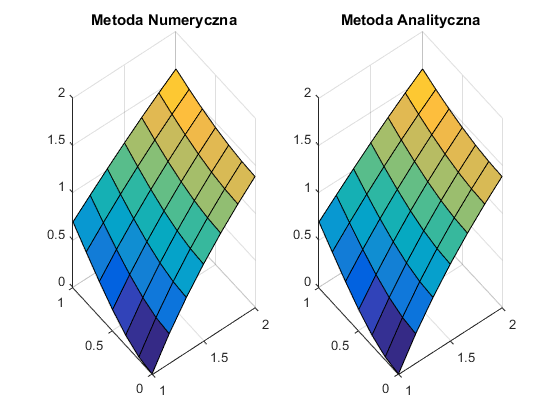
\includegraphics[width=0.78\textwidth]{Lab6/charts/pr/zad1/5.png}
	\end{center}
\end{figure}

Liczba wykonanych iteracji $ = 8 $

Czas wykonywania algorytmu $ = 0.123 s$


Dla n = 15:

\begin{figure}[!ht]
	\begin{center}
		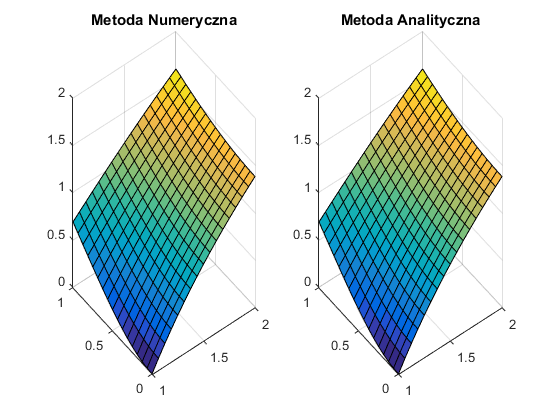
\includegraphics[width=0.78\textwidth]{Lab6/charts/pr/zad1/15.png}
	\end{center}
\end{figure}


Liczba wykonanych iteracji $ = 19 $

Czas wykonywania algorytmu $ = 0.138 s$
\newpage
Dla n = 30:

\begin{figure}[!ht]
	\begin{center}
		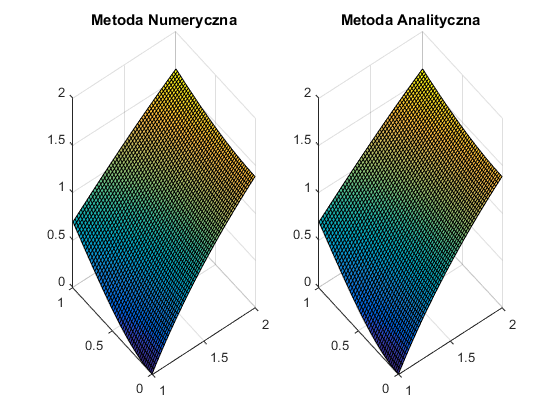
\includegraphics[width=0.8\textwidth]{Lab6/charts/pr/zad1/30.png}
	\end{center}
\end{figure}

Liczba wykonanych iteracji $ = 37 $

Czas wykonywania algorytmu $ = 0.212 s$



Dla n = 50:

\begin{figure}[!ht]
	\begin{center}
		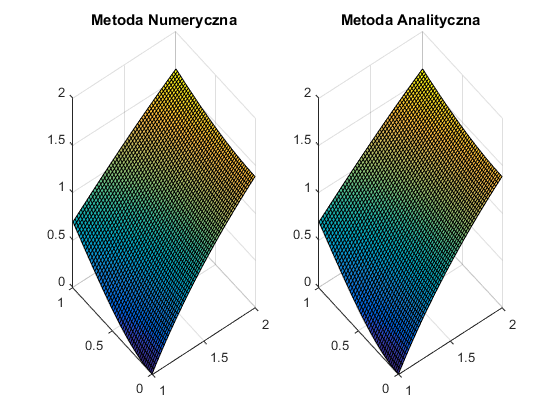
\includegraphics[width=0.8\textwidth]{Lab6/charts/pr/zad1/50.png}
	\end{center}
\end{figure}

Liczba wykonanych iteracji $ = 57 $

Czas wykonywania algorytmu $ = 0.456 s$
\newpage
b)

Dla n = 5:

\begin{figure}[!ht]
	\begin{center}
		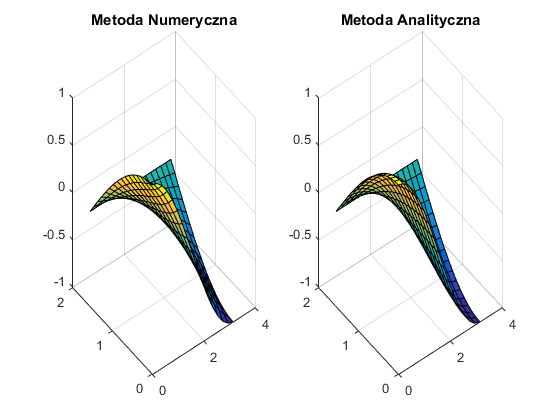
\includegraphics[width=0.8\textwidth]{Lab6/charts/pr/zad2/5.png}
	\end{center}
\end{figure}

Liczba wykonanych iteracji $ = 14 $

Czas wykonywania algorytmu $ = 0.150 s$

Dla n = 15:

\begin{figure}[!ht]
	\begin{center}
		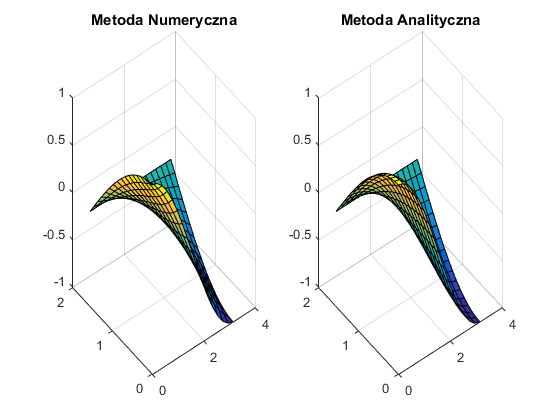
\includegraphics[width=0.8\textwidth]{Lab6/charts/pr/zad2/15.png}
	\end{center}
\end{figure}

Liczba wykonanych iteracji $ = 26 $

Czas wykonywania algorytmu $ = 0.143 s$

Dla n = 30:

\begin{figure}[!ht]
	\begin{center}
		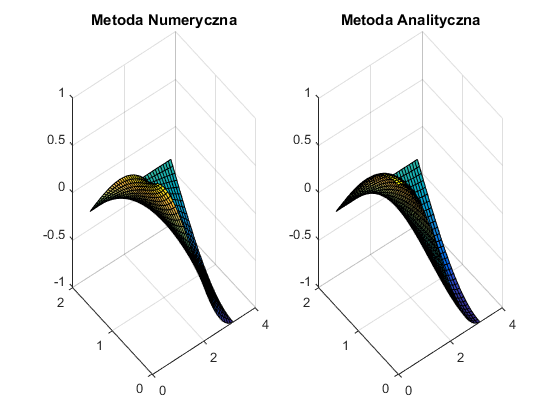
\includegraphics[width=0.8\textwidth]{Lab6/charts/pr/zad2/30.png}
	\end{center}
\end{figure}

Liczba wykonanych iteracji $ = 39 $

Czas wykonywania algorytmu $ = 0.211 s$



Dla n = 50:

\begin{figure}[!ht]
	\begin{center}
		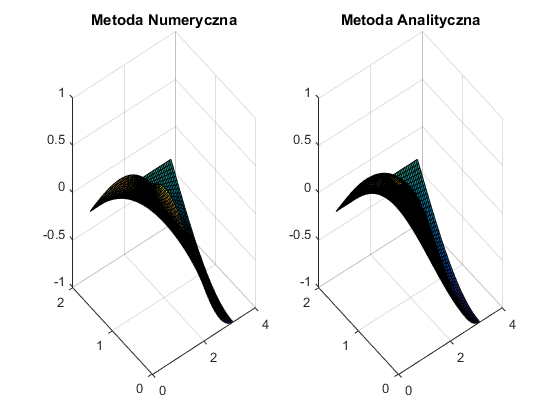
\includegraphics[width=0.8\textwidth]{Lab6/charts/pr/zad2/50.png}
	\end{center}
\end{figure}

Liczba wykonanych iteracji $ = 57 $

Czas wykonywania algorytmu $ = 0.452 s$

\newpage

\subsection{Zestawienie metod iteracyjnych}
\begin{figure}[!ht]
	\begin{center}
		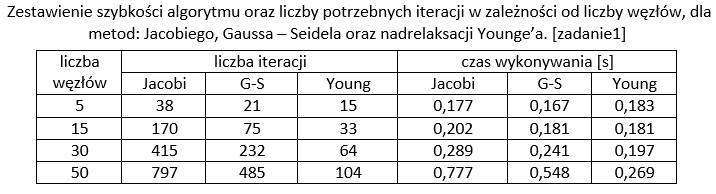
\includegraphics[width=1\textwidth]{Lab6/charts/zestawienie_zad1.png}
	\end{center}
\end{figure}

\begin{figure}[!ht]
	\begin{center}
		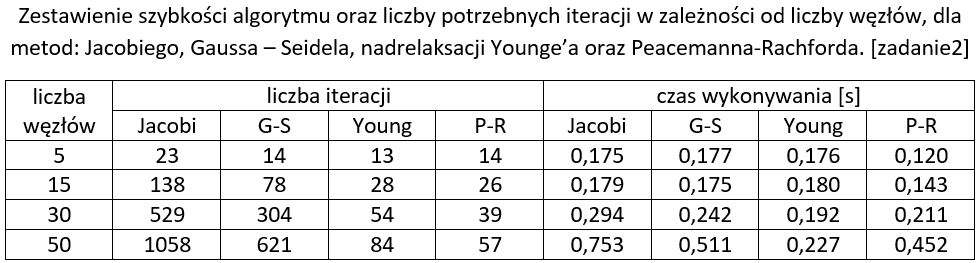
\includegraphics[width=1\textwidth]{Lab6/charts/zestawienie_zad2.png}
	\end{center}
\end{figure}